\chapter{Literature Review}\label{chap:literature}

% \epigraph{\textbf{democracy} \\
%     \emph{de$\cdot$moc$\cdot$ra$\cdot$cy} | \emph{noun} \\
%     A system of government in which power is vested in the people.
% }{}

This chapter is broken into two major sections:

\begin{itemize}
   % \item \emph{Democracies and Electoral Systems}, which reviews domestic and
   %    foreign elections, voter's rights and legal protections, vote casting
   %    devices, the various processes and systems in place for casting votes,
   %    novel electoral systems and experiments, contentious elections, and the
   %    reasons why these contentious elections are regarded as such.

   \item \emph{Internet Voting}, which introduces Internet voting: procedures
      and concepts, and offers a survey of significant Internet voting systems,
      projects, pilots, and experiments.

   \item \emph{End-to-End Verifiability}, which introduces the concept of
      end-to-end verifiable (E2E-V) voting systems, reviews the functionalities
      required to support end-to-end verifiability (technical and
      non-functional), the architectural options available, existing E2E-V
      systems, and common cryptographic techniques available for use in such
      systems.

   % \item \emph{Blockchain Technology}, which reviews the Ethereum blockchain:
   %    its fundamental concepts and abstractions, internal data structures,
   %    algorithms, the Ethereum Virtual Machine (EVM), network topology and
   %    architecture.
\end{itemize}

% Section: Democracies and Electoral Systems
% \section{Democracies and Electoral Systems}

% Democracy is a fundamental birthright for Americans, a cherished blessing
% which serves as the foundation for our freedom. Each generation must nourish
% and foster the processes of their democracy so that future generations may too
% reap the benefits it provides.

% FIXME: All of this seems better suited for the introduction!
Key to democracy is the right to vote. By voting the citizens of a democratic
society can express their will to a governing body. The goal of any voting
system should be to produce an outcome which fairly represents the will of the
people.

Societies have practiced democracy for thousands of years: held elections,
casted votes, and executed on the results. However, technology, and its
applications with respect to voting systems, have developed markedly in that
time. Today the Internet pervades our lives in the form of websites,
applications, peripherals and more --- used for social media, banking,
e-commerce, and everything in-between --- this leads one wonder why it is that
we haven't seen more progress in the form of Internet-based voting.
Constituents, election officials, businesses, counties, states, even entire
countries have requested and experimented with such systems. Internet security
is robust enough to support a \$100 billion industry, e-commerce, which suggests
that an Internet-based voting system is at least plausible.

Contentious election results have been seen both locally and abroad, as well as
issues that cast doubt and concern on the validity of our democratic processes:
voter suppression, gerrymandering, intimidation, ballot stuffing, destruction of
audit material, etc. Internet based voting systems might help to alleviate some
of these concerns. Research on end-to-end verifiable voting has seen much
progress in the past few years. However, Internet voting brings with it an
entirely new set of security risks and concerns that must also be addressed.

The legitimacy of a government depends on public perception. Thus, election
security is a matter of national security. Voters must be certain that their
votes have not been unfairly manipulated or tallied to modify election results,
they must feel that universal suffrage is being upheld, that all those who are
eligible to vote have had the opportunity to do so, that each voter has had
precisely one vote, that each vote is of equal weight, and that the privacy of
each voter has been maintained.

Voting is the means through which we express ourselves; if voters lose faith in
their electoral system they will lose faith in their election results, their
elected leaders, and their democracy. Trustworthy democracy is an ambitious and
worthy goal that every government should strive to realize.

% What follows are a review of various election systems.

\subsection{Voter's Rights and Legislation}
American elections are a massive and complicated undertaking filled with
federal, state, and local legislation. Interestingly, neither the Bill of Rights
nor the US Constitution originally spelled out any right to vote, active
suffrage, for the citizens of its democracy. Indeed, the United States still
does not offer universal suffrage to its citizens, e.g., felons are
disenfranchised. It wasn't until the Fifteenth Amendment was ratified that the
right to vote for citizens and the protections for citizen's right to vote were
finally recognized at a federal level. In total, we have had four separate
amendments to the Constitution which concern voting rights:

\begin{itemize}
  \item Fifteenth Amendment --- Racial suffrage (1870)
    \begin{displayquote}
      The right of citizens of the United States to vote shall not be denied or
      abridged by the United States or by any state on account of race, color,
      or previous condition of servitude.
    \end{displayquote}
    % \textquote{The right of citizens of the United States to vote shall not be denied or abridged by the United States or by any state on account of race, color, or previous condition of servitude.}

  \item Nineteenth Amendment --- Sexual suffrage (1920)
    \begin{displayquote}
      The right of citizens of the United States to vote shall not be denied or
      abridged by the United States or by any on account of sex.
    \end{displayquote}
    % \textquote{The right of citizens of the United States to vote shall not be denied or abridged by the United States or by any on account of sex.}

  \item Twenty-fourth Amendment --- Financial suffrage (1964)
    \begin{displayquote}
      The right of citizens of the United States to vote in any primary or other
      election for President or Vice President, for electors for President or
      Vice President, or for Senator or Representative in Congress, shall not be
      denied or abridged by the United States or any State by reason of failure
      to pay any poll tax or other tax.
    \end{displayquote}
    % \textquote{The right of citizens of the United States to vote in any primary or other election for President or Vice President, for electors for President or Vice President, or for Senator or Representative in Congress, shall not be denied or abridged by the United States or any State by reason of failure to pay any poll tax or other tax.}

  \item Twenty-sixth Amendment --- Age suffrage (1971)
    \begin{displayquote}
      The right of citizens of the United States, who are eighteen years of age
      or older, to vote shall not be denied or abridged by the United States or
      by any State on account of age.
    \end{displayquote}
    % \textquote{The right of citizens of the United States, who are eighteen years of age or older, to vote shall not be denied or abridged by the United States or by any State on account of age.}
\end{itemize}

There are several major pieces of legislation relevant to voter's voting rights.
Many of these statutes provide basic voting rights and others go further to
ensure that these rights are upheld for various demographics via varied
enforcement policies.

\subparagraph{Voting Rights Act}
Although the Fifteenth Amendment of the Constitution was ratified in 1870 it
wasn't until the \emph{Voting Rights Act (VRA)}, passed in 1965, that the
Fifteenth Amendment was actually enforced. The act laid out a number of
provisions used to regulate election administration. Prior to the VRA southern
states would disenfranchise racial minorities via Jim Crow laws, election fraud,
voter restrictions: literacy tests, poll taxes, property-ownership requirements,
moral character tests, requirements that voter registration applicants interpret
particular documents, etc.

\subparagraph{Uniformed and Overseas Citizens Absentee Voting Act}
The \emph{Uniformed and Overseas Citizens Absentee Voting Act (UOCAVA)} was
passed in 1986 to render services to merchant marines, uniformed services, and
other overseas civilians. Specifically, UOCAVA mandates that overseas and
military voters be able to remotely register and vote in federal elections. The
\emph{Federal Voting Assistance Program (FVAP)}, established under the
\emph{Department of Defense (DOD)}, provides voter assistance, tools, and
education to overseas voters so that they are able to vote from anywhere in the
world.

\subparagraph{National Voter Registration Act}
The \emph{National Voter Registration Act (NVRA)}, also known the
\emph{Motor Voter Act}, was federal law passed in 1993 that came into effect
in 1995. The goal of NRVA was to increase voter registration, enhance voter
participation, protect election security, and ensure states maintain accurate
voter rolls. This was done by combining voter registration with obtaining a
driver's license.

\begin{displayquote}
  The NVRA effectively forced every state to offer voter registration in
  combination with the single civic act performed almost universally by American
  adults --- obtaining a driver’s license.
\end{displayquote}

% \blockquote{The NVRA effectively forced every state to offer voter
% registration in combination with the single civic act performed almost
% universally by American adults --- obtaining a driver’s license.}

\subparagraph{Help America Vote Act}
The \emph{Help America Vote Act (HAVA)}, passed in 2002, was legislation passed to
lower barriers disabled people encountered while attempting to vote. HAVA also
aimed to improve vote auditing after a large number of ballots in the 2000
election were rejected. HAVA recommended that all election systems use
\emph{Verifiable Voter Paper Audit Trail (VVPAT)} and worked to create statewide
voter registration lists and identification requirements.

HAVA was also responsible for the formation of the United States \emph{Election
Assistance Commission (EAC)}. The EAC is responsible for testing, certifying,
and decertifying voting equipment; developing voting machine standards; and
administering funds to states so that they become HAVA compliant.

The EAC requested that the \emph{National Institute of Standards and Technology
(NIST)} create a \emph{Voluntary Voting System Guidelines (VVSG)} which cover
equipment, documentation, and testing requirements of voting machines.

\begin{displayquote}
  The purpose of the Voluntary Voting System Guidelines is to provide a set of
  specifications and requirements against which voting systems can be tested to
  determine if they provide all the basic functionality, accessibility and
  security capabilities required to ensure the integrity of voting systems. The
  VVSG specifies the functional requirements, performance characteristics,
  documentation requirements, and test evaluation criteria for the national
  certification of voting systems.
\end{displayquote}

HAVA also established provisional ballots for states that don't allow same-day
registration. Provisional ballots allow voters to cast a ballot on election day
if the voter feels they're entitled to vote but are not listed as being
registered. The ballot is counted after the voter's eligibility has been
verified with the goal being that no voter is turned away who should have
otherwise been able to vote.

\subparagraph{Military and Overseas Voter Empowerment Act}
The \emph{Military and Overseas Voter Empowerment Act (MOVE)}, passed in 2009,
amended UOCAVA and other statues to provide further protections to eligible
citizens. Specifically the act aimed to reduce the number of ballots that are
not counted due to late receipt. MOVE accomplishes this by requiring that states
send absentee ballots no later that 45 days prior to election day. MOVE goes
further by requiring that all registration material and blank ballots be
available electronically as well as removes requirements regarding notarization
on voting applications and ballots.

\subparagraph{Voter Empowerment Act}
The \emph{Voter Empowerment Act (VEA)} is meant to improve antiquated voter
registration, ensure access to ballots, preserve the integrity of the voting
system, further prohibit deceptive practices, protect voting rights, and demand
accountability from election administration.

\subsection{Voting Procedures, Technologies, and Availability}
Voting procedure varies depending on state legislation. Here we review early
voting, remote voting, and Internet voting by state. Remote voting is a form of
early voting and Internet voting a form of remote voting.

\paragraph{Early Voting}
\emph{Early voting} is a service which allows voters to cast ballots before
election day during a specified time frame at a polling location. Some states
offer early voting through \emph{in-person absentee voting}: a voter receives a
ballot through mail or internet, marks said ballot, then casts their vote at an
official polling location before Election Day.

Early voting has become a popular means of voting for American citizens. In the
1980s fewer that 5\% of ballots cast in the general election were cast before
election day, by 2000 16\% percent of votes for president were cast early, and
by 2012 the number of votes casted early had risen to at least 31\%.

% ### Arguments
Proponents of early voting argue that early voting makes the voting process more
convenient for citizens, thus increasing voter turnout. Voters would have more
flexibility to work around children, jobs, doctor's appointments, out of state
trips, as well as be able to avoid long lines on election day.

Critics argue that those concerns are less important when compared to the risks
it presents.

\begin{displayquote}
   Citizens should vote with a common base of information about candidates. If
   they vote over a period of weeks before Election Day, they vote based on the
   knowledge available on a scattering of different dates.
\end{displayquote}

\subparagraph{State Breakdown of Early Voting Availability}

% ### State Breakdown
\begin{itemize}
  \item 34 states and the District of Columbia allow any qualified voter to vote
    early without excuse or justification, see
    Table~\ref{tab:pre-election-voting}.

  \item 3 states are remote/early voting exclusively (by mail), see
    Table~\ref{tab:pre-election-voting}.
\end{itemize}

\paragraph{Remote Voting}
\emph{Remote voting}, in contrast to early voting, is any form of voting where
ballots are not marked and cast at an official polling place. Remote voting is
also known as \emph{absentee voting}. The medium through which a marked absentee
ballot is returned to election officials depends on the state.

% ### Arguments
Remote voting offers flexibility above and beyond early voting. Remote voting
allows voters to vote from the comfort of their own homes, overseas, and even
from space. However, there are risks associated with remote voting:
voter intimidation, vote buying, vote manipulation, etc.

\begin{displayquote}
   Growing use of absentee voting has turned this area of voting into the most
   likely opportunity for election fraud now encountered by law enforcement
   officials. These cases are especially difficult to prosecute, since the
   misuse of a voter’s ballot or the pressure on voters occurs away from the
   polling place or any other outside scrutiny. These opportunities for abuse
   should be contained, not enlarged.
\end{displayquote}

% ### State Breakdown
% \subparagraph{Remote Voting by State}
\subparagraph{State Breakdown of Remote Voting Availability}

\begin{itemize}
  \item 27 states and the District of Columbia permit any qualified voter to
    vote absentee, without offering an excuse, via postal service.
    Table~\ref{tab:pre-election-voting}

  \item 20 states require an excuse to remote vote.
    Table~\ref{tab:pre-election-voting}

  \item 3 states are remote/early voting exclusively (by mail).
    Table~\ref{tab:pre-election-voting}
\end{itemize}

\paragraph{Voting Procedure Availability by State}

\begin{center}
    \scriptsize
    \begin{longtabu} to \textwidth{@{} X[1.1,l] X[c] X[0.01] X[c] X[c] X[c] X[c] @{}}
        \caption{Pre-Election Day Voting}\label{tab:pre-election-voting} \\
        \toprule
        \taburowcolors{white..white}
        State                       & \multicolumn{1}{c}{In-Person}         && \multicolumn{4}{c}{By Mail} \\
                                      \cmidrule{2-2}                           \cmidrule{4-7}
                                    & Early Voting                          && No-Excuse Absentee                    & Absentee; Excuse Required             & All-Mail Voting           & Permanent Absentee Status \\
        \midrule
        \taburowcolors{white..gray!15}
        \endfirsthead%

        \toprule
        \taburowcolors{white..white}
        State                       & \multicolumn{1}{c}{In-Person}         && \multicolumn{4}{c}{By Mail} \\
                                      \cmidrule{2-2}                           \cmidrule{4-7}
                                    & Early Voting                          && No-Excuse Absentee                    & Absentee; Excuse Required             & All-Mail Voting           & Permanent Absentee Status \\
        \midrule
        \taburowcolors{white..gray!15}
        \endhead%

        Alabama                     &                                       &&                                       & \textbullet{}                         &                           & \\
        Alaska                      & \textbullet{}                         && \textbullet{}                         &                                       & (1)                       & \\
        Arizona                     & \textbullet{}                         && \textbullet{}                         &                                       & (1)                       & \textbullet{} \\
        Arkansas                    & \textbullet{}                         &&                                       & \textbullet{}                         & (1)                       & \\
        California                  & \textbullet{}                         && \textbullet{}                         &                                       & (1)                       & \textbullet{} \\
        Colorado                    &                                       &&                                       &                                       & \textbullet{}             & \\
        Connecticut                 &                                       &&                                       & \textbullet{}                         &                           & \textbullet{} \\
        Delaware                    &                                       &&                                       & \textbullet{}                         &                           & \\
        D.C.                        & \textbullet{}                         && \textbullet{}                         &                                       &                           & \textbullet{} \\
        Florida                     & \textbullet{}                         && \textbullet{}                         &                                       & (1)                       & \\
        Georgia                     & \textbullet{}                         && \textbullet{}                         &                                       &                           & \\
        Hawaii                      & \textbullet{}                         && \textbullet{}                         &                                       & (1)                       & \textbullet{} \\
        Idaho                       & (2)                                   && \textbullet{}                         &                                       & (1)                       & \\
        Illinois                    & \textbullet{}                         && \textbullet{}                         &                                       &                           & \\
        Indiana                     & (2)                                   &&                                       & \textbullet{}                         &                           & \\
        Iowa                        & (2)                                   && \textbullet{}                         &                                       &                           & \\
        Kansas                      & \textbullet{}                         && \textbullet{}                         &                                       & (1)                       & \\
        Kentucky                    &                                       &&                                       & \textbullet{}                         &                           & \\
        Louisiana                   & \textbullet{}                         &&                                       & \textbullet{}                         &                           & \\
        Maine                       & (2)                                   && \textbullet{}                         &                                       &                           & \\
        Maryland                    & \textbullet{}                         && \textbullet{}                         &                                       & (1)                       & \\
        Massachusetts               & (3)                                   &&                                       & \textbullet{}                         &                           & \\
        Michigan                    &                                       &&                                       & \textbullet{}                         &                           & \\
        Minnesota                   & (2)                                   && \textbullet{}                         &                                       & (1)                       & \textbullet{} \\
        Mississippi                 &                                       &&                                       & \textbullet{}                         &                           & \\
        Missouri                    &                                       &&                                       & \textbullet{}                         & (1)                       & \\
        Montana                     & (2)                                   && \textbullet{}                         &                                       & (1)                       & \textbullet{} \\
        Nebraska                    & \textbullet{}                         && \textbullet{}                         &                                       & (1)                       & \\
        Nevada                      & \textbullet{}                         && \textbullet{}                         &                                       & (1)                       & \\
        New Hampshire               &                                       &&                                       & \textbullet{}                         &                           & \\
        New Jersey                  & (2)                                   && \textbullet{}                         &                                       & (1)                       & \textbullet{} \\
        New Mexico                  & \textbullet{}                         && \textbullet{}                         &                                       & (1)                       & \\
        New York                    &                                       &&                                       & \textbullet{}                         &                           & \\
        North Carolina              & \textbullet{}                         && \textbullet{}                         &                                       &                           & \\
        North Dakota                & \textbullet{}                         && \textbullet{}                         &                                       & (1)                       & \\
        Ohio                        & (2)                                   && \textbullet{}                         &                                       &                           & \\
        Oklahoma                    & (2)                                   && \textbullet{}                         &                                       &                           & \\
        Oregon                      &                                       &&                                       &                                       & \textbullet{}             & \\
        Pennsylvania                &                                       &&                                       & \textbullet{}                         &                           & \\
        Rhode Island                &                                       &&                                       & \textbullet{}                         &                           & \\
        South Carolina              &                                       &&                                       & \textbullet{}                         &                           & \\
        South Dakota                & (2)                                   && \textbullet{}                         &                                       &                           & \\
        Tennessee                   & \textbullet{}                         &&                                       & \textbullet{}                         &                           & \\
        Texas                       & \textbullet{}                         &&                                       & \textbullet{}                         &                           & \\
        Utah                        & \textbullet{}                         && \textbullet{}                         &                                       &                           & \textbullet{} \\
        Vermont                     & (2)                                   && \textbullet{}                         &                                       &                           & \\
        Virginia                    &                                       &&                                       & \textbullet{}                         &                           & \\
        Washington                  &                                       &&                                       &                                       & \textbullet{}             & \\
        West Virginia               & \textbullet{}                         &&                                       & \textbullet{}                         &                           & \\
        Wisconsin                   & (2)                                   && \textbullet{}                         &                                       &                           & \\
        Wyoming                     & (2)                                   && \textbullet{}                         &                                       &                           & \\

        \taburowcolors{white..white}
        \cmidrule{1-7}

        TOTAL                       & 34 states + DC                        && 27 states + DC                        & 20 states                             & 3 states                  & 8 states + DC \\
        \bottomrule
    \end{longtabu}
    \begin{enumerate}[leftmargin=5mm,topsep=0mm]
      \item Certain elections may be held entirely by mail. The circumstances
        under which all-mail elections are permitted vary from state to state.

      \item Although these states do not have Early Voting in the traditional
        sense, within a certain period of time before an election they do allow
        a voter to apply in person for an absentee ballot (without an excuse)
        and cast that ballot in one trip to an election official’s office. This
        is often known as ``in-person absentee'' voting.

      \item Massachusetts has Early Voting only during even-year November
        elections, beginning in 2016. Currently it does not permit Early Voting
        in primaries or municipal elections.
    \end{enumerate}
\end{center}

% \textbf{Source:} National Conference of State Legislatures, January 2016.
% http://www.ncsl.org/research/elections-and-campaigns/absentee-and-early-voting.aspx


\paragraph{Electronic Voting}
\emph{Electronic voting}, also referred to as \emph{e-voting}, is the use of
electronic systems to cast and/or count votes. There are two major categories of
electronic voting worth considering:

\begin{itemize}
  \item \emph{Direct Recording Electronic (DRE) voting machines}, which provide
    mechanisms for voters to digitally mark and cast their ballot; votes which
    are cast via DRE voting machine are recorded electronically in the voting
    machine's memory for later tallying.

  \item \emph{Optical scan voting systems}, which do not provide a mechanism for
    voter's to cast a ballot, unlike DRE voting machines, but instead provide an
    electronic means of counting physical ballots which have already been cast.
    This functionality is provided via optical scanning technology, much like
    Scantrons in the academic world, and allows election officials to tally
    ballots much more quickly than possible when compared to manual
    ballot-tallying procedures.
    % thus provide initial elections results earlier, and certify election
    % results more quickly
\end{itemize}

% ### Arguments
% \subparagraph{Advantages}
Proponents of electronic voting argue that e-voting provides a faster, more
transparent, more secure, and more accurate form of voting. Other argued
benefits include greater ballot language support, increased support and
independence for handicapped people, lower costs, and the ability to entirely
prevent spoiled ballots.

% \subparagraph{Disadvantages}
Critics of electronic voting argue that the promises of e-voting have repeatedly
fallen short of expectations. Security researchers have demonstrated methods of
attacking various e-voting machines to manipulate votes casted or the tallying
process itself. As a result most states no longer offer e-voting without a
\emph{Verifiable Voter Paper Audit Trail (VVPAT)}. Proponents and vendors of
electronic voting systems have argued that their systems are rigorously tested;
however, security experts have challenged not only the rigorousness of the
available testing procedures, but also the notion that testing procedures are a
sufficient measure of a system's security.

\begin{displayquote}
   Election law in most states requires that all voting systems—whether
   electronic or not—be qualified by an authorized federally licensed laboratory
   known as an Independent Testing Authority (ITA), and then submitted to the
   state for certification. The ostensible purpose of these procedures it to
   make sure that the voting system meets the voluntary federal voting system
   standards promulgated by the FEC (and in the future, by NIST), and that they
   conform to the state’s election laws. It is tempting to place a lot of faith
   in certification procedures as a means for preventing security failures. We
   believe such faith is unwarranted. We argue that even a lengthy,
   conscientious testing and examination program by the most qualified people
   cannot give us the necessary security guarantees. In fact, in general, no
   process can, since in most cases the problem of establishing that a program
   meets any particular security requirement is known to be fundamentally
   unsolvable.
\end{displayquote}

\begin{displayquote}
   There are fundamental limits to what testing can accomplish; it is a truism
   of the software world that while testing can be used to verify that bugs and
   security vulnerabilities are present, it can never prove that they are
   absent.
\end{displayquote}

\begin{displayquote}
   Contrary to many people’s intuition, it is unlikely in the extreme that
   anyone, whether on the development team or not, would detect malicious logic
   that was deliberately disguised by a clever programmer, no matter how much
   effort was put into the search. It is much easier to hide a needle in a
   haystack than to find it.
\end{displayquote}

\paragraph{Internet Voting}
\emph{Internet voting} is defined as any form of voting where a marked ballot is
transfered over a network, this includes transfer via fax, email, or web
application (fax being included because of the widespread proliferation and
usage of Internet-based fax machines).

There have been many attempts to bring about online voting in the US and abroad.
Over \$100 million in federal funding and decades of research and development
has been spent on internet voting systems.

\begin{displayquote}
   In 2000 there were several other experiments with Internet voting in U.S.
   public elections. In some cases the votes counted officially; in others they
   did not. The largest and most well-known was the Arizona Democratic
   presidential primary, conducted by election.com (whose assets were acquired
   in 2003 by Accenture) in March of that year, in which approximately 85,000
   votes were cast and counted. The Reform Party national primary was also
   conducted over the Internet that summer, as were various nonbinding Internet
   voting experiments in some counties of Washington, California, Arizona and
   elsewhere.
\end{displayquote}

% ### Arguments
Internet voting has the potential to provide all of the benefits of early,
remote, and electronic voting, but also inherits all of their risks, and some.
The major additional risk is that Internet voting exposes the entire system to
remote attack from anywhere in the world and the possibility for large-scale
attacks.

The general consensus of research initiatives and academic research is that
Internet voting is fundamentally impossible to accomplish while maintaining
voter privacy, audit trails, and preventing large scale attacks.

\begin{displayquote}
   it is currently not possible to ensure the security, privacy, auditability
   and integrity of ballots cast over the Internet.

   \dots

   federal researchers determined that secure online voting is not currently
   feasible

   \dots

   The conclusive evidence that online voting cannot yet be done securely led
   the federal government to abandon its effort to develop a secure online
   voting system for the military in 2014.
\end{displayquote}

\begin{displayquote}
   It is reasonable to assume that the shortcomings of ITAs with respect to DREs
   will carry over to their certification of Internet voting.
\end{displayquote}

``A comment on the May 2007 DoD report on Voting Technologies for UOCAVA
Citizens'' made the following arguments against such voting systems:

\begin{itemize}
  \item Paperless (non-VVPAT) voting systems have been widely criticized: closed
    source software, insufficient security, insider attack potential, and no
    VVPAT.\

  \item Cyber attack potential: insider attacks, denial of service attacks,
    spoofing, automated vote buying, viral attacks, etc.

  \item Attacks could occur at a large-scale and launched by individual,
    corporate, or state actors that may lie outside the reach of US law. Attacks
    could result in widespread or selective voter disenfranchisement, vote
    buying/selling, vote switching, etc. These attacks are capable of being
    perpetrated without detection.

  \item These vulnerabilities cannot be eliminated without a wholesale redesign
    and replacement of both the internet and PC.\

  \item Seemingly successful Internet voting systems may appear to work
    flawlessly, promoting expansion of an insecure system.

  \item Not detecting a successful attack does not mean that one has not
    occurred.

  \item Because the threat of large-scale cyber attacks is so great, ``we
    recommend against any Internet voting until both the Internet and the
    world's home computer infrastructure have been fundamentally redesigned.''
\end{itemize}

% Sub-Section: Electoral System Design
%\subsection{Contentious Elections}
Despite having had thousands of years to improve on our election systems we
continue to see contentious election results both locally and abroad. What
follows are some of the more egregious and contentious election results.

\paragraph{American Elections}
\subparagraph{Bush vs Gore (2000 --- United States)}


\subparagraph{Trump vs Clinton (2016 --- United States)}
\begin{displayquote}
  ``A 58 percent majority of Clinton supporters say they accept Trump's
  election, while 33 percent do not. Questions about Trump's victory are
  passionate --- 27 percent of Clinton supporters feel ``strongly'' he did not
  win legitimately.''
\end{displayquote}

\paragraph{Foreign Elections}
\subparagraph{Gortari vs Cárdenas (1988 --- Mexico)}

\todo{Add back the Contentious Elections sub-section once it has been improved.}

% Sub-Section: Electoral System Design
\subsection{Design Principles}

\todo{
  This section was taken from the Methods, it should be covered in the
  Literature Review, referenced from the Methods, addressed again in the
  Discussion, and briefly mentioned in the Conclusion.
}

We borrow design principles from ``Electoral System Design: The New
International IDEA Handbook'' which were outlined in Chapters 2 and 3.

\subparagraph{Representation} We wish to achieve fair representation. What
constitutes fair representation will largely depend on the greater democratic
framework and the constitutes of that framework. Our electoral system should
translate votes into winning choices in a way that accurately and fairly
represents the will of the people while also being flexible enough to allow for
configuration and modification appropriate for various governance structures.

\subparagraph{Transparency} Our electoral system should be as transparent as
possible, preferably end-to-end verifiable. The winners, losers, and electorate
must be able to trust that the results of an election were achieved
legitimately.

\subparagraph{Inclusiveness} Our electoral system should support full suffrage
(active and passive) as well as universal suffrage. The mechanisms of the
electoral system should not be biased such that any group is discriminated
against. Designing an electoral system with inclusiveness in mind results in
governance with a stronger sense of legitimacy and wider participation and
willingness to participate by the electorate.

\paragraph{International Standards} There is no universally agreed upon
standards, but most would agree upon the following standards.

\begin{enumerate}[label=\Large$\square$]
  \item Elections should be free, fair, and periodic.
  \item Universal adult suffrage should be supported.
  \item Ballot secrecy should be preserved and constituents should be free
    from coercion.
  \item A commitment to the principle of ``one person, one vote.''
\end{enumerate}

\paragraph{Design Checklist}
We also borrow a design checklist from the ``Electoral System Design: The New
International IDEA Handbook.''

\begin{enumerate}[label=\Large$\square$]
  \item Is the system clear and comprehensible?
  \item Has context been taken into account?
  \item Is the system appropriate for the time?
  \item Are the mechanisms for future reform clear?
  \item Does the system avoid underestimating the electorate?
  \item Is the system as inclusive as possible?
  \item Was the design process perceived to be legitimate?
  \item Will the election results be seen as legitimate?
  \item Are unusual contingencies taken into account?
  \item Is the system financially and administratively sustainable?
  \item Will the voters feel motivated to participate?
  \item Is a competitive party system encouraged?
  \item Does the system fit into a holistic constitutional framework?
  \item Will the system help alleviate conflict rather than exacerbate it?
\end{enumerate}



% Section: Voting
% \section{Internet Voting}\label{sec:internet-voting}
Internet voting, sometimes referred to as \emph{remote electronic voting}, is a
system of voting where voters are able to cast their votes over the Internet.

% \subsection{Procedure}
% \todo{
%   This doesn't need to be a subsection, just mention it at the start of the
%   Internet Voting section.
% }
\paragraph{Procedure}
The U.S.\ Vote Foundation describes the typical phases involved in conducting an
Internet based election as follows:\cite{e2e-viv}

\begin{enumerate}
  \item \emph{Setup}, during which election officials gather voter information,
    identify election issues and races, design ballots, etc.

  \item \emph{Distribution}, during which election materials are distributed to
    voters: ballots, credentials, voting instructions, etc.

  \item \emph{Voting}, during which voters mark their ballots.

  \item \emph{Casting}, where voters finalize and submit their ballots and
    election officials receive said ballots.

  \item \emph{Tallying}, where election officials count votes, tabulate results,
    and announce winners.

  \item \emph{Auditing}, where (as necessary) vote results are evaluated for
    incorrect results.
\end{enumerate}
% \todo{cite: The Future of Voting — Chapter 3.1}
% cite: The Future of Voting - Chapter 3.1

% \subsection{Requirements}
\paragraph{Requirements}
The requirements for an Internet-based voting system are the same as those for
any other voting system; it must be \emph{secure}, \emph{correct}, and
\emph{private}.
% \todo{Complete section.}

\subsection{Survey of Internet Voting Systems}

In September of 2011 the \emph{Election Assistance Commission (EAC)} published
\emph{``A Survey of Internet Voting,''} which offered a broad review of various
Internet voting systems used between the years of 2000 and
2011.\cite{internet-voting-survey} In total, the survey reviews 30 Internet
voting systems used for elections and primaries, by various parties and
governments, at various levels of government: national, state, and local.

% The survey defines internet voting as,
%
% \begin{displayquote}
%   any system where the voter's ballot selections are transmitted over the
%   Internet from a location other than a polling place to the entity conducting
%   the election.
% \end{displayquote}

% cite: A Survey of Internet Voting Systems - EAC
% https://www.eac.gov/sites/default/files/eac_assets/1/28/SIV-FINAL.pdf

% \begin{description}[style=multiline,font=\normalfont,leftmargin=2cm]
%   \item[2000] Alaska sponsored by the Democratic National Party,
%   \item[2000] Arizona 2000 by the Arizona Democratic Party, and
%   \item[2000] VOI by the FVAP,
%
%   \item[2004] Michigan by the Michigan Democratic Party,
%   \item[2004] SERVE by the FVAP,
%
%   \item[2005/2007/2009/2011] Estonia,
%
%   \item[2008] Democrats Abroad by Democrats Abroad,
%   \item[2008/2010] Arizona 2008/2010 by Arizona Secretary of State's Office,
%   \item[2008] ODBP by Okaloosa County Supervisor of Elections,
%
%   \item[2009] Honolulu by the City of Honolulu,
%
%   \item[2010] District of Columbia by the DC Board of Elections and Ethics,
%   \item[2010] Oregon by the Independent Party of Oregon,
%   \item[2010] West Virginia by the West Virginia Secretary of State,
% \end{description}

\subsubsection{Voting Over the Internet (VOI) --- 2000}

% \subparagraph{Background}
In 1986, the \emph{Uniformed and Overseas Citizens Absentee Voting Act (UOCAVA)}
was passed to render services to merchant marines, uniformed services, and other
overseas civilians. Broadly, UOCAVA mandates that overseas and military
voters be able to remotely register and vote in federal elections, and
designates the Secretary of Defense as the executive agent responsible for
implementing its provisions. Thus, under the \emph{Department of Defense
(DoD)}, the \emph{Federal Voting Assistance Program (FVAP)} was established  to
provide voter assistance, tools, and education to overseas voters with the goal
of enabling overseas voters to vote from anywhere in the world. In pursuit of
this goal, FVAP established procedures for delivering election materials through
domestic, military, and foreign postal systems.

% \paragraph{Objectives and Motivations}
In an effort to eliminate some of the weaknesses inherit in postal systems,
primarily transit times and unreliable delivery guarantees, FVAP established the
\emph{Voting Over the Internet (VOI)} project.

\begin{displayquote}
  ``The pilot project was designed to examine the feasibility of using the
  Internet for remote registration and voting in an effort to overcome the time
  and distance barriers faced by UOCAVA voters. `This was the first time that
  binding votes were cast over the Internet for federal, state, and local
  offices, including the President and Members of
  Congress.'{}''\cite{internet-voting-survey,voi-assessment-report}
\end{displayquote}
% cite: A Survey of Internet Voting Systems - EAC

% \paragraph{Architecture}
The VOI architecture consisted of 3 major components, as illustrated in
Figure~\ref{fig:voi-architecture}:

\begin{itemize}
  \item Citizen infrastructure: any workstation or personal computer with
    Internet access that was available to the voter.

  \item FVAP infrastructure: VOI systems maintained by FVAP, namely the FVAP
    server, which hosted the server-side VOI software, various intrusion
    detection systems, networking infrastructure, and administrative
    workstations.

  \item Local Election Official (LEO) infrastructure: systems managed by
    LEOs, namely servers running VOI software and workstations to interact with
    said software.
\end{itemize}

\begin{figure}[H]
    \centering
    \includegraphics[width=\textwidth]{03-literature/figures/internet-voting/voi/voip}
    % \includesvg[width=\textwidth]{03-literature/figures/internet-voting/voi/voi.svg}
    % \input{03-literature/figures/internet-voting/voi/voi2.pdf_tex}
    % 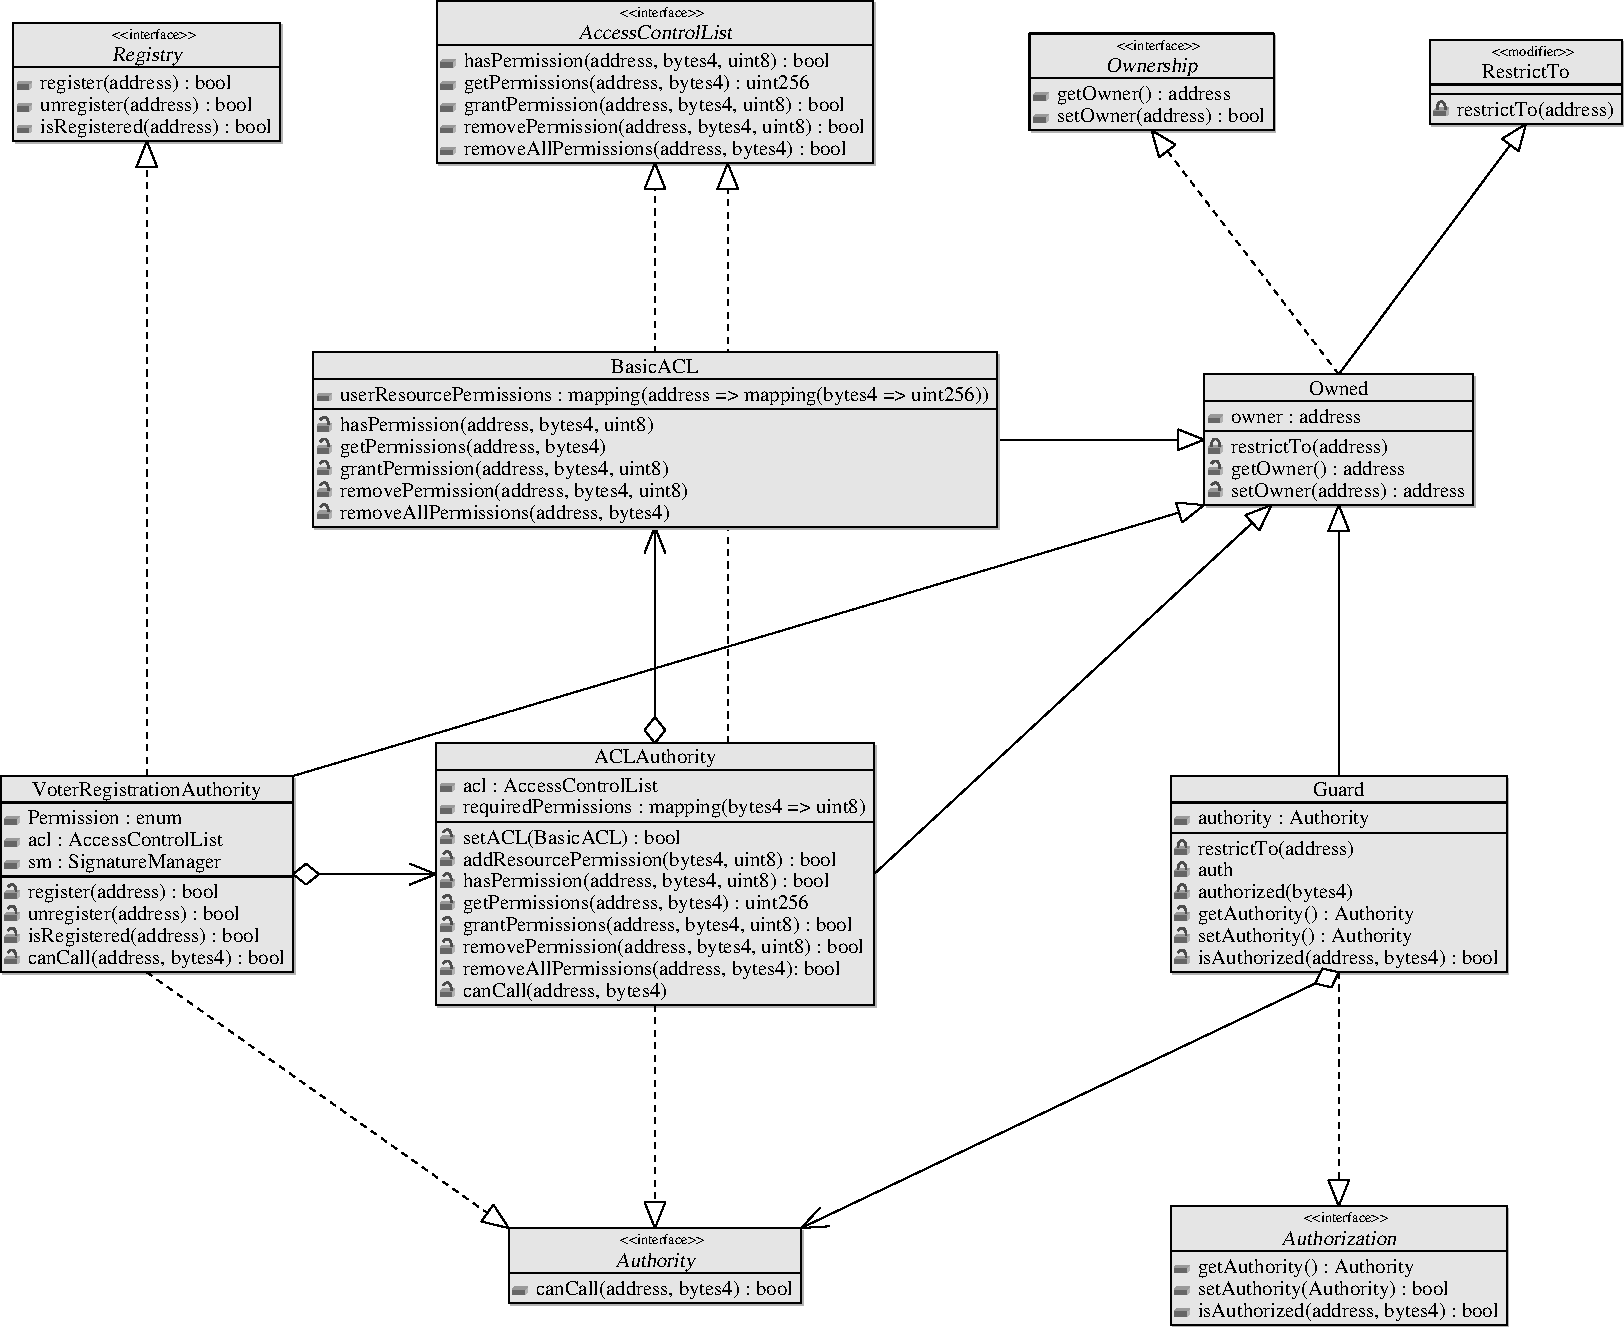
\includegraphics[width=\textwidth]{figures/authorization/figure}
    % \includestandalone[width=\textwidth]{\fig{authorization}}
    \caption{VOI System Architecture~\cite{voi-assessment-report}}\label{fig:voi-architecture}% \label{fig:authorization}
\end{figure}
% cite: Department of Defense Washington Headquarters Services Federal Voting
% cite: https://www.fvap.gov/uploads/FVAP/Reports/voi.pdf
% Assistance Program Voting Over the Internet Pilot Project Assessment Report

\subparagraph{Citizen Infrastructure}
FVAP mailed a CD-ROM to participants containing VOI software, this came in the
form of a Netscape Navigator browser plug-in which provided a graphical user
interface to cast ballots and communicate with the VOI server-side components.
% cite: https://www.fvap.gov/uploads/FVAP/Reports/voi.pdf

% \begin{displayquote}
%   The citizen workstation was the computing platform used by participating
%   citizens to access the Pilot System from their residences or workplaces. The
%   performance requirements for the workstations were intentionally modest to
%   ensure that most existing personal computers would be compatible. The
%   minimum requirements were that the citizen workstation run a Microsoft
%   Windows 95/98 operating system, have a connection to the Internet, and have
%   the Netscape Navigator browser (Version 4.05 or higher, with strong
%   encryption) installed to provide a graphical user interface to the VOI
%   System. Macintosh or UNIX platforms could not be used, nor could Microsoft's
%   Internet Explorer browser. Custom software to enable VOI-specific
%   functionality, in the form of a browser plug-in, was included on a CD-ROM
%   sent to each citizen by the FVAP\@. The CD-ROM also included the strong
%   encryption (128 bit) version of Netscape Navigator for those citizens who
%   needed to upgrade their browser software to be compatible.
% \end{displayquote}

\subparagraph{FVAP Infrastructure}
The FVAP infrastructure consisted of the FVAP server hosting the VOI software,
various networking and power redundancy components to support the server, two
network intrusion detection systems, a server hosting software for creating
electronic ballots, and an administrative workstation for interacting with the
FVAP server. The collective functionalities which this infrastructure provided
included voter authentication, ballot routing to LEO infrastructure, and ballot
creation.

% \begin{displayquote}
% The FVAP server segment was the central component of the VOI System, providing
% the link between the citizen workstations and the LEO servers. The FVAP server
% segment included several different computing platforms, network communication
% components (router, hub), and other components, including a printer, an
% uninterruptible power supply, and a modem for paging system operations and
% maintenance staff. The FVAP segment included the FVAP server, two intrusion
% detection systems, the E-Ballot Tool server, and the FVAP administrative
% workstation.The administrative workstation is a personal computer running a
% Netscape Navigator browser client and is the principal interface to the FVAP
% server for system performance monitoring activities. The two intrusion
% detection system components were positioned on the outside and inside of the
% filtering router to monitor network activities and identify suspicious
% behavior. The intrusion detection system located outside the router is not
% depicted in the system architecture diagram. These two components, along with
% the filtering router and configuration changes to the FVAP server's Microsoft
% Windows NT™ operating system all combined to make the FVAP segment an
% important security barrier protecting the Pilot System.
%
% \emph{FVAP Server}
% The FVAP server included a highly reliable computer hardware server, its
% operating system,database management software, application server software,
% and the VOI custom-developed software. From a functional perspective, the FVAP
% server identified and authenticated users, allowed users to transfer
% Electronic Federal Post Card Applications (EFPCAs) and E-Ballots to and from
% the LEO servers, and performed ``postmarking'' functions. The content of all
% transactions passed through the FVAP server in encrypted form so only the
% addressing information could be read for communications routing purposes.
%
% \emph{E-Ballot Tool Server}
% The E-Ballot Tool server was located within the FVAP server segment security
% architecture and access to it was restricted to specified LEO staff via an
% access control list. This server was dedicated to hosting the E-Ballot Tool
% software. The LEOs used this software to build their electronic ballots. After
% all the component files for the ballots were defined, the LEO would copy those
% associated with a specific ballot style to a floppy disk and upload them to
% the LEO server. No ballots were stored on the E-Ballot Tool server.
% \end{displayquote}

\subparagraph{Local Election Official Infrastructure}
Each LEO site managed a server running VOI software which connected over the
Internet with the FVAP-maintained VOI server and a workstation which allowed
LEOs to perform administrative operations with the server.

% \begin{displayquote}
% Each LEO site had a server that provided connectivity only from the FVAP server
% via the Internet to transmit or receive EFPCAs, E-Ballots, and status messages.
% Each LEO segment included the server hardware platform, the Microsoft Windows NT
% operating system, the VOI custom software, a printer, a removable storage media
% unit, uninterruptible power supply, and network communications devices. Like the
% FVAP segment, each LEO segment had an additional workstation for administration
% of the LEO server.
% \end{displayquote}

% \paragraph{Outcome}
The VOI pilot successfully served 84 volunteers across 4 states. Administrators
did not detect any intrusions into the system during its operation. However, the
DoD acknowledged in their assessment report that one of the major shortcomings
of the pilot was its small sample size, and, that the incentive to attack such a
system would increase as the number of participants
increased.\cite{voi-assessment-report} A future security panel criticized the
VOI system for taking the position that, ``the citizen's workstation is outside
the security perimeter of the system,'' noting that it effectively ignores some
of the most serious kinds of attacks which the system is vulnerable
to.\cite{serve-analysis} On the topic of remote internet voting the DoD
assessment report expressed the following:

\begin{displayquote}[][]
  ``[remote internet voting] is subject to the same security concerns as the
  current VOI System. For this reason, we cannot recommend this alternative as
  an immediate follow-on development to the VOI
  Pilot.\cite{voi-assessment-report}''
\end{displayquote}

%%
% Secure Electronic Registration and Voting Experiment (SERVE) — 2004
%%

\subsubsection{Secure Electronic Registration and Voting Experiment (SERVE) --- 2004}

% In 2002, as directed by Congress and as an immediate follow-on development to
% the VOI pilot, the DoD began work on a remote Internet voting project.

% \subparagraph{Background}
In 2002, following the VOI project, Congress instructed the DoD to carry out a
larger demonstration project, ``under which absent uniformed services voters are
permitted to cast ballots in the regularly scheduled general election for
Federal office.''\cite{serve-bill} To fulfill this mandate FVAP contracted
Accenture to build \emph{The Secure Electronic Registration and Voting
Experiment} (SERVE).

% \paragraph{Objectives and Motivations}
SERVE was built under the United States' Department of Defense's (DoD) Federal
Voting Assistance Program (FVAP) to be deployed for the 2002 or 2004 elections.
Broadly, the motivations behind SERVE were to produce an Internet-based voting
system to reduced barriers to voting for Americans living overseas; specifically
the objectives of the project were to:

\begin{enumerate}
  \item ``assess whether the use of electronic voting technology could improve the
    voting participation success rate for UOCAVA
    citizens,''\cite{dod-expanding-electronic-voting} and

  \item ``assess the potential impact on state and local election administration
    of an automated alternative to the conventional by-mail process of absentee
    registration and voting.''\cite{dod-expanding-electronic-voting}
\end{enumerate}

Fifty counties covering 7 states were targeted for participation and the system was
designed to handle both the registration and voting process.

\paragraph{Architecture}
SERVE shared many architectural-similarities to VOI which are reflected in the
SERVE architecture diagram seen in Figure~\ref{fig:serve-architecture}\@:

\begin{itemize}
  \item SERVE was designed as a web-based service which a voter could connect to
    via web browser.

  \item LEOs managed a local server which could be used to interact with
    the central SERVE system.

  \item The central SERVE system, which performed the bulk of the system
    processing, was maintained by FVAP and stored voter information until the
    appropriate LEO server downloaded it.
\end{itemize}
% to be stored by the central SERVE system that was to be maintained by FVAP\@.

The system was described as consisting of eight integrated subsystems:
Identification and Authentication; Common Services; Voter Registration; Election
Administration; Ballot Definition; Voting; Download and Decryption; and
Tabulation.

\begin{figure}[H]
    \centering
    \includegraphics[width=\textwidth]{03-literature/figures/internet-voting/serve/architecture}
    \caption{SERVE System Architecture~\cite{internet-voting-survey}}\label{fig:serve-architecture}% \label{fig:authorization}
\end{figure}

%  would
% handle identification, registration, authentication, and ballot casting
% procedures. Ballots would be encrypted with LEO  which allowed them to access voter data and encrypted ballots which were

To participate one had to have a military ID (a Common Access Card), or could
enroll in the SERVE system by presenting face-to-face proof of citizenship to a
SERVE official. Once enrolled and registered, a participant could vote via a web
browser through the SERVE site. Figure~\ref{fig:serve-voting-protocol} outlines
the protocol used for casting a ballot through the SERVE web application.

\begin{figure}[H]
    \centering
    \includegraphics[width=0.8\textwidth]{03-literature/figures/internet-voting/serve/protocol}
    \caption{SERVE Voting Protocol~\cite{internet-voting-survey}}\label{fig:serve-voting-protocol}% \label{fig:authorization}
\end{figure}

% \paragraph{Outcome}
SERVE received harsh criticism from independent system reviewers, members of the
\emph{Security Peer Review Group (SPRG)}, academics and industry professionals
who were assembled by FVAP to evaluate the system. A group of these members
independently publicized concerns regarding the security of the system and
Internet-based voting systems more broadly.\cite{serve-analysis}

% \subparagraph{Vulnerabilities}
The report published notes that SERVE suffers from a number of vulnerabilities
and goes into great detail regarding the risks these vulnerabilities pose and
the complexity of performing various attacks to take advantage of these
vulnerabilities. The report noted:\cite{serve-analysis}

\begin{enumerate}
  \item Lack of voter-verified audit trails and vulnerabilities to insider
    attacks. Vulnerabilities in software are difficult to find and intentionally
    obfuscated vulnerabilities are even more so. The essentially unauditable
    nature of electronic voting systems necessitate some form of voter-verified
    audit trail.

  \item Privacy. Several system design issues were identified which would allow
    LEOs or SERVE administrators to tie a ballot to a voter's identity.

  \item Vote Buying/Selling. The nature of Internet voting makes selling
    credentials for voting systems a very real possibility.

  \item Intimidation. Voter intimidation is a problem which all remote voting
    systems must contend with, this problem extends to Internet voting systems.

  \item Large-Scale Impact. Electronic voting machines, if compromised, might
    enable attackers to modify or damage tens or hundreds of thousands of
    ballots. Internet voting systems face this same issue, except on a much
    larger scale; the entire system essentially acts as a single electronic
    voting machine, significantly increasing the scale of impact if compromised.
    Paper-based systems do not face these same exposures.

  \item Too Many Potential Attacks. Electronic systems present a large attack
    surface, exposure to the Internet presents even more. Mitigation of all of
    the kinds of attacks possible would not be feasibility.

  \item Many Sources of Attacks. Elections held over the Internet are vulnerable
    to attacks from around the globe; nation-state entities, terrorists,
    individual hackers and more would all have the ability to attack system.

  \item Undetectable Attacks. Electronic systems make detecting attacks
    extremely difficult and the lack of a detected attack on a system does not
    prove that no attack occurred.

  \item On-screen Electioneering. Many states prevent campaigning within some
    distance of a polling place; however, no such laws exist to prevent ISPs,
    web browsers, or other entities from displaying ads to voters.
\end{enumerate}

% The details of the vulnerabilities reported
% are discussed in further detail in Section~\ref{section:shared-weaknesses},
% however, the report notes:

In addition the report had this to say about future attempts at building
Internet voting systems:

\begin{displayquote}
  ``Like the proponents of SERVE, we believe that there should be better support
  for voting for our military overseas. Still, we regret that we are forced to
  conclude that the best course is not to field the SERVE system at all. Because
  the danger of successful, large-scale attacks is so great, we reluctantly
  recommend shutting down the development of SERVE immediately and not
  attempting anything like it in the future until both the Internet and the
  world's home computer infrastructure have been fundamentally redesigned, or
  some other unforeseen security breakthroughs appear.''\cite{serve-analysis}
\end{displayquote}

In response to these criticisms and concerns documented in this report, the
then-Deputy Secretary of Defense Paul Wolfowitz decided that the SERVE project
would not go forward as planned for the 2004 election, effectively killing the
project.\cite{dod-expanding-electronic-voting} Three years later the DoD
published a report which downplayed the criticisms and concerns published by the
SPRG members.\cite{dod-expanding-electronic-voting} In reaction to this DoD
report, the members of the SPRG independently publicized a response which
criticized the report for downplaying the concerns laid out in their initial
security analysis of SERVE, and further reiterated their concerns regarding
Internet voting. The members of the SPRG noted again that the issues faced by
SERVE are ones which are not capable of being fixed by a better design or
architecture of Internet voting systems, because the fundamental issues are ones
which could only be fixed by redesigning both the Internet and personal
computers.\cite{comment-on-dod-report}

% \subsubsection{Integrated Voting Alternative Site (IVAS)}
% September 2006

% Interim Voting Assistance System
% https://graphics8.nytimes.com/packages/pdf/national/2006_IVAS_report.pdf

% Integrated Voting Alternative Site
% https://www.fvap.gov/uploads/FVAP/Reports/ivas06.pdf
% \todo{What does IVAS stand for? A: It stands for both.}
% \todo{Complete section.}

\subsubsection{D.C. Digital Vote-by-Mail System (DVBM) --- 2010}

% \subparagraph{Background}
In 2009 the \emph{Military and Overseas Voter Empowerment Act (MOVE)} was
passed. This act amended UOCAVA and other statutes to provide further protections
to eligible citizens. Specifically the act aimed to reduce the number of ballots
which are not counted due to late receipt. MOVE accomplishes this by requiring
that states send absentee ballots no later that 45 days prior to election day.
MOVE goes further by requiring that all registration material and blank ballots
be available electronically and removes requirements regarding notarization on
voting applications and ballots.\cite{MOVE}

% \begin{displayquote}
%   In 2010, Washington, D.C.\ developed an Internet voting pilot project that was
%   intended to allow overseas absentee voters to cast their ballots using a
%   website.
%   % https://jhalderm.com/pub/papers/dcvoting-fc12.pdf
% \end{displayquote}

% \paragraph{Objectives and Motivations}
In search of a solution to improve their compliance with the MOVE act,
Washington's District of Columbia Board of Elections and Ethics (DCBOEE/BOEE)
planned to launch an Internet voting system, the D.C. Digital Vote-by-Mail
(DVBM) system, for use in the November 2010 general election. The project was
developed in partnership with the Open Source Digital Voting (OSDV) Foundation's
TrustTheVote project, who viewed the project as a mostly academic
effort.\cite{trust-the-vote-dc-pilot} The system was slated to be operational in
time for the November 2010 general election and aimed to provide two primary
functionalities:\cite{internet-voting-survey,dc-voting-system}
\begin{enumerate}
  \item allow voters to electronically access voting materials
  \item allow voters to optionally cast their ballot over the internet
\end{enumerate}

% \paragraph{Architecture}
The DVBM architecture, illustrated in Figure~\ref{fig:dvbm-architecture}, was
developed as a web application using the Ruby on Rails framework; was hosted
using the Apache web server; used MySQL as its database technology, which stored
the global election state (voters' names, addresses, etc.); and used the
underlying (Linux) filesystem to store encrypted ballots cast by voters. When
the voting phase of the election was complete, election officials would transfer
the encrypted ballots to an air-gapped computer for decryption and printing.
Printed ballots would be counted alongside other mail-in absentee
ballots.\cite{dc-voting-system}

\begin{figure}[H]
    \centering
    \includegraphics[width=\textwidth]{03-literature/figures/internet-voting/dc/architecture}
    % \includesvg[width=\textwidth]{03-literature/figures/internet-voting/voi/voi.svg}
    % \input{03-literature/figures/internet-voting/voi/voi2.pdf_tex}
    % 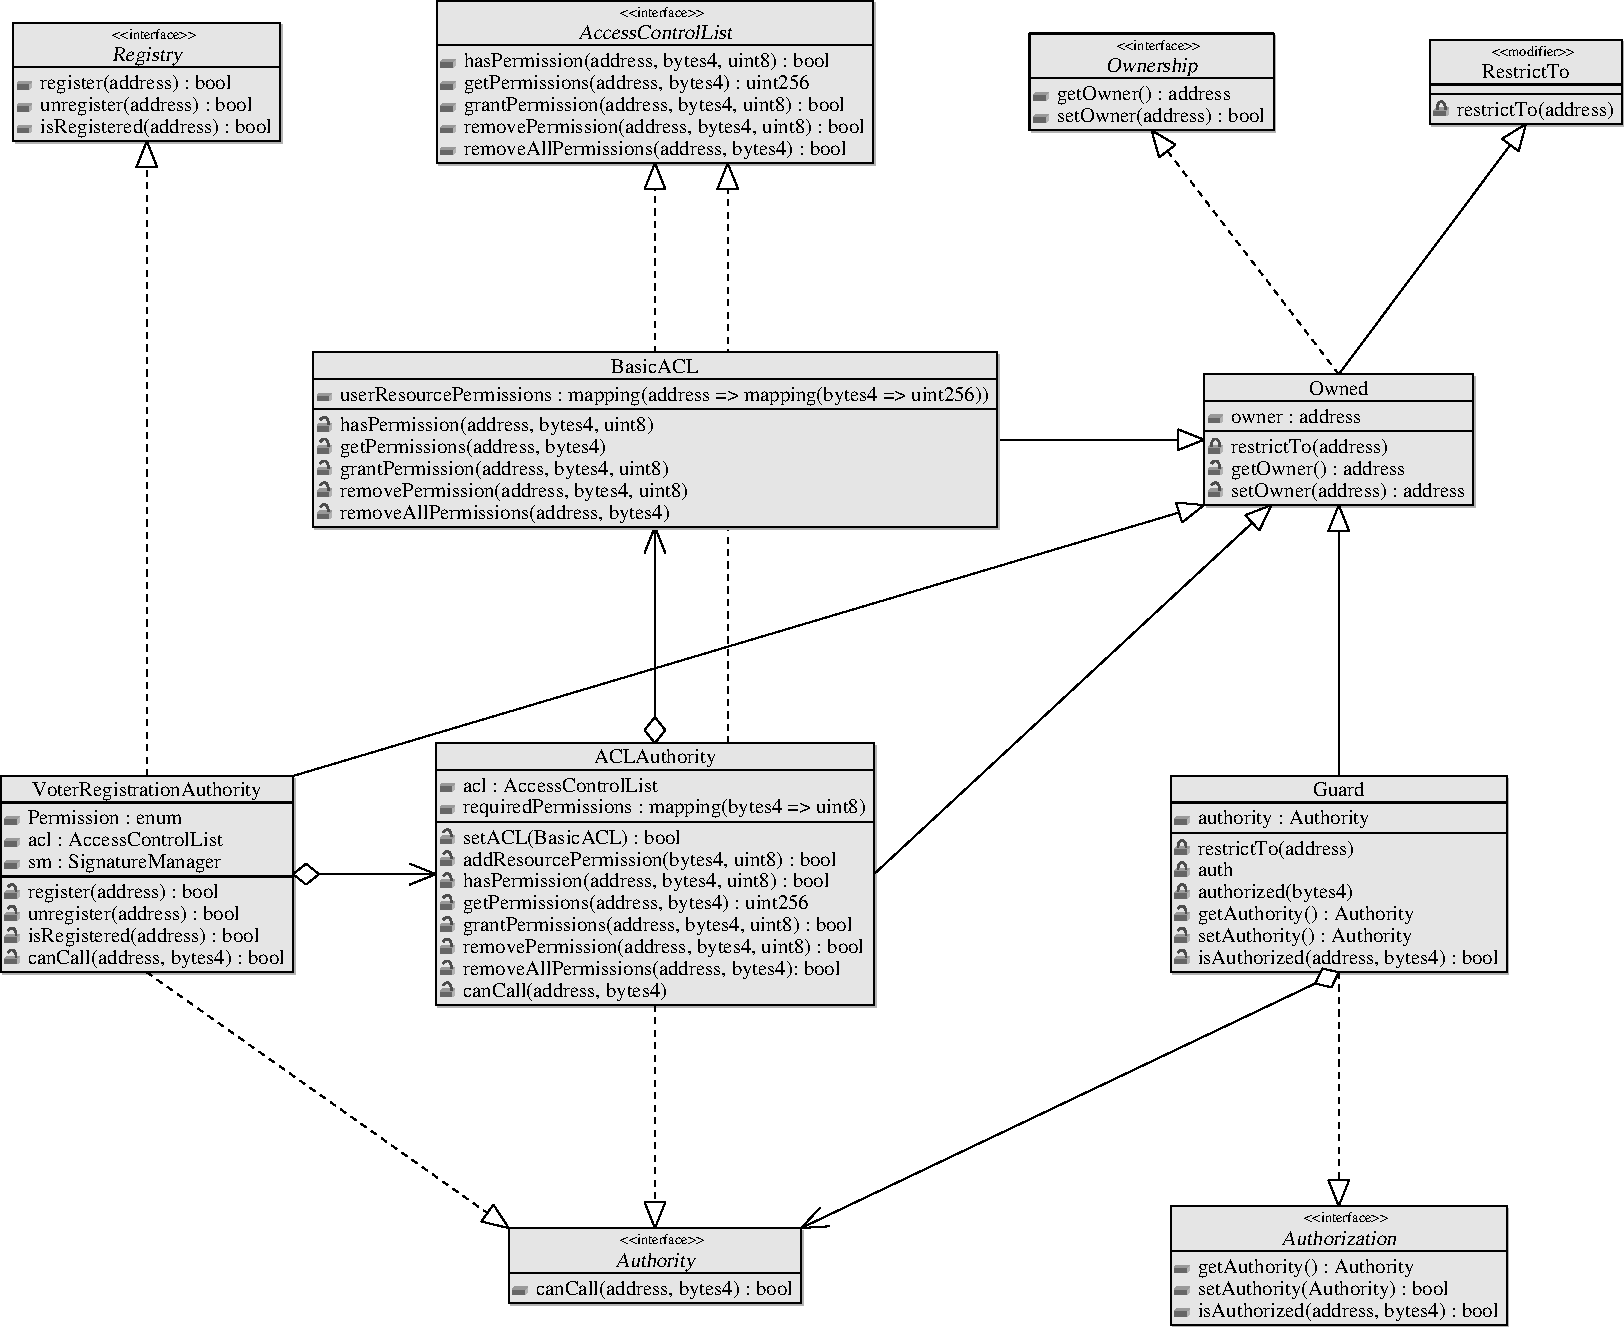
\includegraphics[width=\textwidth]{figures/authorization/figure}
    % \includestandalone[width=\textwidth]{\fig{authorization}}
    \caption{DVBM System Architecture~\cite{dc-voting-system}}\label{fig:dvbm-architecture}% \label{fig:authorization}
\end{figure}

Prior to the official launch of the system the BOEE opted to conduct a mock
election where members of the public, researchers, and hackers alike were
invited to to test the functionality of the system, discover vulnerabilities,
and attempt to compromise the security, reliability, and availability of the
system.\cite{internet-voting-survey,dc-voting-system,trust-the-vote-dc-pilot}

% \paragraph{Outcome}
Within 48 hours of the system going live researchers from The University of
Michigan, playing the role of an attacker, demonstrated a number of
vulnerabilities and attacks on on the system and managed to gained near-complete
control of the election server. Their intrusion was not detected for nearly 2
days.\cite{dc-voting-system}
% Prior to its launch election officials held a mock election to test the security
% of the system, inviting researchers and hackers alike to attempt to compromise
% the security, reliability, and availability of the system. A number of attacks
% were demonstrated and researchers were able to:

Demonstrated vulnerabilities included being able to:
\begin{itemize}
  \item penetrate the network of the election software
  \item determine voter's identities
  \item locate unencrypted ballots, thus mapping voter's identities to their
    personal votes
  \item modify ballots
  \item cast fake ballots
  \item modify the election system software itself
\end{itemize}

Once election officials became aware of the attack, the mock election was
suspended, five days ahead of schedule, citing ``usability issues.'' Election
officials later confirmed that they were unable to detect the attack or network
presence using their intrusion detection system. Due to the test results, the
portion of the system which allowed for ballots to be submitted over the
Internet was not used.\cite{dc-voting-system}

\subsubsection{Estonia --- 2005}
Estonia began using Internet voting in 2005\cite{internet-voting-survey}; in the
2015 Estonian parliamentary elections, 30.5\% of all voters voted over the
Internet. Estonia maintains what is likely the most advanced national
identification cards in the world. Estonian IDs are part of a \emph{Public Key
Infrastructure (PKI)} where IDs serve as smart cards which possess two RSA key
pairs: one for signing and one for authentication; these cryptographic functions
are performed directly on the card. The signatures produced by these IDs are
used extensively throughout the country and are considered legally binding.
These cryptographic IDs allow Estonia to provide voter authentication
capabilities that cannot be reproduced in the US.\ Despite the advanced
authentication capabilities that Estonia is able to achieve, researchers in 2014
devised a number of attacks that could be performed on the Estonian voting
system to spoil ballots, damage ballot secrecy, and steal or drop votes. The
researchers also criticized the transparency and operational security of the
system, noting that videos of the administration processes --- provided for
transparency purposes --- recorded administrators entering root passwords,
revealed network credentials which had been posted on a wall, and showed
administrators using USB drives containing personal files to move sensitive
election materials between systems.\cite{estonia}

% \subsection{Shared Weaknesses}\label{section:shared-weaknesses}
% There are a number of shared weaknesses and vulnerabilities exposed across these
% internet voting systems which the systems incur due to the underlying
% architecture of the systems, their Internet, the personal computer, and remote
% voting.
%
% \begin{enumerate}
%   \item Lack of voter-verified audit trails.
%   \item Vulnerabilities to insider attacks.
%   \item Privacy.
%   \item Vote Buying/Selling.
%   \item Intimidation.
%   \item Large-Scale Impact.
%   \item Too Many Potential Attacks.
%   \item Many Sources of Attacks.
%   \item Undetectable Attacks.
%   \item On-screen Electioneering.
% \end{enumerate}

% \todo{
%   Should I add a shared weaknesses section here and remove some of the
%   demonstrated attacks from the individual systems?
% }


% Section: Internet Voting
\section{Internet Voting}\label{sec:internet-voting}
Internet voting, sometimes referred to as \emph{remote electronic voting}, is a
system of voting where voters are able to cast their votes over the Internet.

% \subsection{Procedure}
% \todo{
%   This doesn't need to be a subsection, just mention it at the start of the
%   Internet Voting section.
% }
\paragraph{Procedure}
The U.S.\ Vote Foundation describes the typical phases involved in conducting an
Internet based election as follows:\cite{e2e-viv}

\begin{enumerate}
  \item \emph{Setup}, during which election officials gather voter information,
    identify election issues and races, design ballots, etc.

  \item \emph{Distribution}, during which election materials are distributed to
    voters: ballots, credentials, voting instructions, etc.

  \item \emph{Voting}, during which voters mark their ballots.

  \item \emph{Casting}, where voters finalize and submit their ballots and
    election officials receive said ballots.

  \item \emph{Tallying}, where election officials count votes, tabulate results,
    and announce winners.

  \item \emph{Auditing}, where (as necessary) vote results are evaluated for
    incorrect results.
\end{enumerate}
% \todo{cite: The Future of Voting — Chapter 3.1}
% cite: The Future of Voting - Chapter 3.1

% \subsection{Requirements}
\paragraph{Requirements}
The requirements for an Internet-based voting system are the same as those for
any other voting system; it must be \emph{secure}, \emph{correct}, and
\emph{private}.
% \todo{Complete section.}

\subsection{Survey of Internet Voting Systems}

In September of 2011 the \emph{Election Assistance Commission (EAC)} published
\emph{``A Survey of Internet Voting,''} which offered a broad review of various
Internet voting systems used between the years of 2000 and
2011.\cite{internet-voting-survey} In total, the survey reviews 30 Internet
voting systems used for elections and primaries, by various parties and
governments, at various levels of government: national, state, and local.

% The survey defines internet voting as,
%
% \begin{displayquote}
%   any system where the voter's ballot selections are transmitted over the
%   Internet from a location other than a polling place to the entity conducting
%   the election.
% \end{displayquote}

% cite: A Survey of Internet Voting Systems - EAC
% https://www.eac.gov/sites/default/files/eac_assets/1/28/SIV-FINAL.pdf

% \begin{description}[style=multiline,font=\normalfont,leftmargin=2cm]
%   \item[2000] Alaska sponsored by the Democratic National Party,
%   \item[2000] Arizona 2000 by the Arizona Democratic Party, and
%   \item[2000] VOI by the FVAP,
%
%   \item[2004] Michigan by the Michigan Democratic Party,
%   \item[2004] SERVE by the FVAP,
%
%   \item[2005/2007/2009/2011] Estonia,
%
%   \item[2008] Democrats Abroad by Democrats Abroad,
%   \item[2008/2010] Arizona 2008/2010 by Arizona Secretary of State's Office,
%   \item[2008] ODBP by Okaloosa County Supervisor of Elections,
%
%   \item[2009] Honolulu by the City of Honolulu,
%
%   \item[2010] District of Columbia by the DC Board of Elections and Ethics,
%   \item[2010] Oregon by the Independent Party of Oregon,
%   \item[2010] West Virginia by the West Virginia Secretary of State,
% \end{description}

\subsubsection{Voting Over the Internet (VOI) --- 2000}

% \subparagraph{Background}
In 1986, the \emph{Uniformed and Overseas Citizens Absentee Voting Act (UOCAVA)}
was passed to render services to merchant marines, uniformed services, and other
overseas civilians. Broadly, UOCAVA mandates that overseas and military
voters be able to remotely register and vote in federal elections, and
designates the Secretary of Defense as the executive agent responsible for
implementing its provisions. Thus, under the \emph{Department of Defense
(DoD)}, the \emph{Federal Voting Assistance Program (FVAP)} was established  to
provide voter assistance, tools, and education to overseas voters with the goal
of enabling overseas voters to vote from anywhere in the world. In pursuit of
this goal, FVAP established procedures for delivering election materials through
domestic, military, and foreign postal systems.

% \paragraph{Objectives and Motivations}
In an effort to eliminate some of the weaknesses inherit in postal systems,
primarily transit times and unreliable delivery guarantees, FVAP established the
\emph{Voting Over the Internet (VOI)} project.

\begin{displayquote}
  ``The pilot project was designed to examine the feasibility of using the
  Internet for remote registration and voting in an effort to overcome the time
  and distance barriers faced by UOCAVA voters. `This was the first time that
  binding votes were cast over the Internet for federal, state, and local
  offices, including the President and Members of
  Congress.'{}''\cite{internet-voting-survey,voi-assessment-report}
\end{displayquote}
% cite: A Survey of Internet Voting Systems - EAC

% \paragraph{Architecture}
The VOI architecture consisted of 3 major components, as illustrated in
Figure~\ref{fig:voi-architecture}:

\begin{itemize}
  \item Citizen infrastructure: any workstation or personal computer with
    Internet access that was available to the voter.

  \item FVAP infrastructure: VOI systems maintained by FVAP, namely the FVAP
    server, which hosted the server-side VOI software, various intrusion
    detection systems, networking infrastructure, and administrative
    workstations.

  \item Local Election Official (LEO) infrastructure: systems managed by
    LEOs, namely servers running VOI software and workstations to interact with
    said software.
\end{itemize}

\begin{figure}[H]
    \centering
    \includegraphics[width=\textwidth]{03-literature/figures/internet-voting/voi/voip}
    % \includesvg[width=\textwidth]{03-literature/figures/internet-voting/voi/voi.svg}
    % \input{03-literature/figures/internet-voting/voi/voi2.pdf_tex}
    % 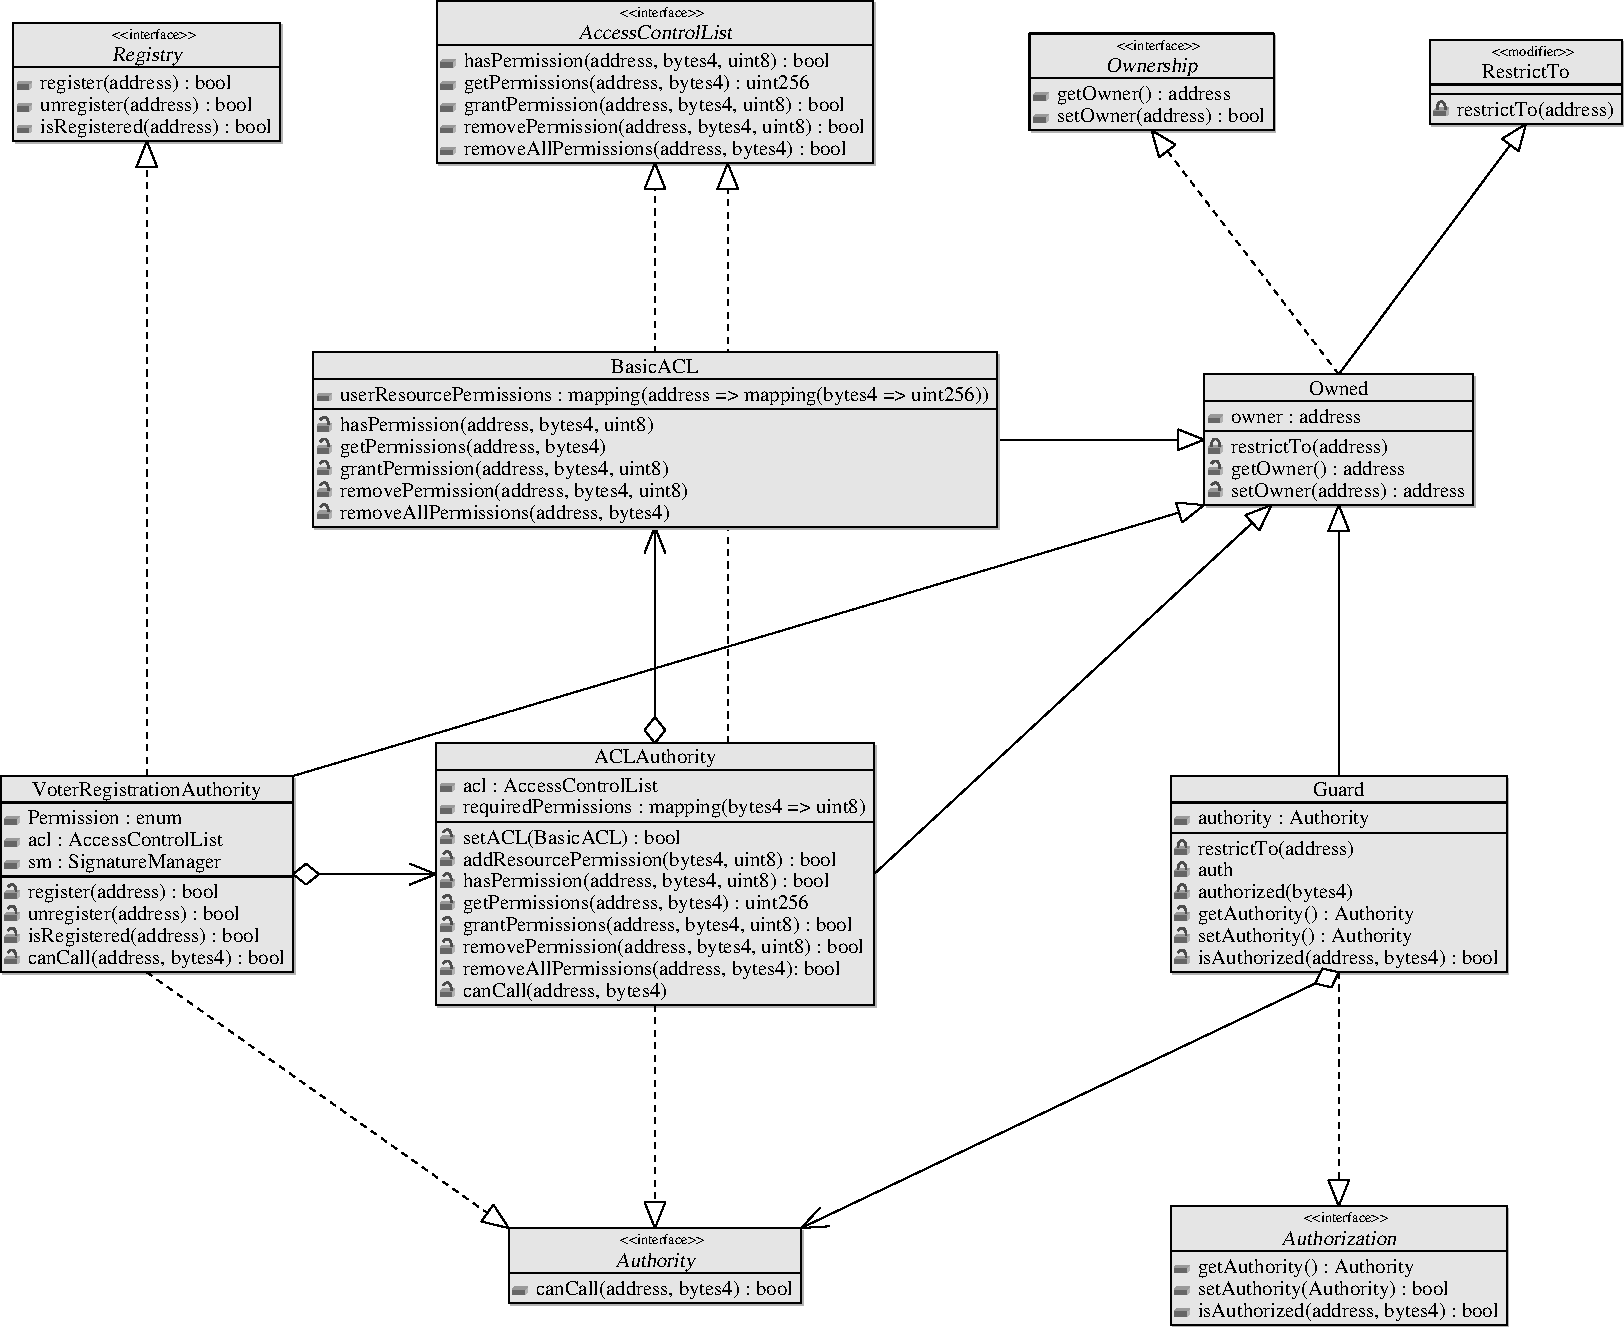
\includegraphics[width=\textwidth]{figures/authorization/figure}
    % \includestandalone[width=\textwidth]{\fig{authorization}}
    \caption{VOI System Architecture~\cite{voi-assessment-report}}\label{fig:voi-architecture}% \label{fig:authorization}
\end{figure}
% cite: Department of Defense Washington Headquarters Services Federal Voting
% cite: https://www.fvap.gov/uploads/FVAP/Reports/voi.pdf
% Assistance Program Voting Over the Internet Pilot Project Assessment Report

\subparagraph{Citizen Infrastructure}
FVAP mailed a CD-ROM to participants containing VOI software, this came in the
form of a Netscape Navigator browser plug-in which provided a graphical user
interface to cast ballots and communicate with the VOI server-side components.
% cite: https://www.fvap.gov/uploads/FVAP/Reports/voi.pdf

% \begin{displayquote}
%   The citizen workstation was the computing platform used by participating
%   citizens to access the Pilot System from their residences or workplaces. The
%   performance requirements for the workstations were intentionally modest to
%   ensure that most existing personal computers would be compatible. The
%   minimum requirements were that the citizen workstation run a Microsoft
%   Windows 95/98 operating system, have a connection to the Internet, and have
%   the Netscape Navigator browser (Version 4.05 or higher, with strong
%   encryption) installed to provide a graphical user interface to the VOI
%   System. Macintosh or UNIX platforms could not be used, nor could Microsoft's
%   Internet Explorer browser. Custom software to enable VOI-specific
%   functionality, in the form of a browser plug-in, was included on a CD-ROM
%   sent to each citizen by the FVAP\@. The CD-ROM also included the strong
%   encryption (128 bit) version of Netscape Navigator for those citizens who
%   needed to upgrade their browser software to be compatible.
% \end{displayquote}

\subparagraph{FVAP Infrastructure}
The FVAP infrastructure consisted of the FVAP server hosting the VOI software,
various networking and power redundancy components to support the server, two
network intrusion detection systems, a server hosting software for creating
electronic ballots, and an administrative workstation for interacting with the
FVAP server. The collective functionalities which this infrastructure provided
included voter authentication, ballot routing to LEO infrastructure, and ballot
creation.

% \begin{displayquote}
% The FVAP server segment was the central component of the VOI System, providing
% the link between the citizen workstations and the LEO servers. The FVAP server
% segment included several different computing platforms, network communication
% components (router, hub), and other components, including a printer, an
% uninterruptible power supply, and a modem for paging system operations and
% maintenance staff. The FVAP segment included the FVAP server, two intrusion
% detection systems, the E-Ballot Tool server, and the FVAP administrative
% workstation.The administrative workstation is a personal computer running a
% Netscape Navigator browser client and is the principal interface to the FVAP
% server for system performance monitoring activities. The two intrusion
% detection system components were positioned on the outside and inside of the
% filtering router to monitor network activities and identify suspicious
% behavior. The intrusion detection system located outside the router is not
% depicted in the system architecture diagram. These two components, along with
% the filtering router and configuration changes to the FVAP server's Microsoft
% Windows NT™ operating system all combined to make the FVAP segment an
% important security barrier protecting the Pilot System.
%
% \emph{FVAP Server}
% The FVAP server included a highly reliable computer hardware server, its
% operating system,database management software, application server software,
% and the VOI custom-developed software. From a functional perspective, the FVAP
% server identified and authenticated users, allowed users to transfer
% Electronic Federal Post Card Applications (EFPCAs) and E-Ballots to and from
% the LEO servers, and performed ``postmarking'' functions. The content of all
% transactions passed through the FVAP server in encrypted form so only the
% addressing information could be read for communications routing purposes.
%
% \emph{E-Ballot Tool Server}
% The E-Ballot Tool server was located within the FVAP server segment security
% architecture and access to it was restricted to specified LEO staff via an
% access control list. This server was dedicated to hosting the E-Ballot Tool
% software. The LEOs used this software to build their electronic ballots. After
% all the component files for the ballots were defined, the LEO would copy those
% associated with a specific ballot style to a floppy disk and upload them to
% the LEO server. No ballots were stored on the E-Ballot Tool server.
% \end{displayquote}

\subparagraph{Local Election Official Infrastructure}
Each LEO site managed a server running VOI software which connected over the
Internet with the FVAP-maintained VOI server and a workstation which allowed
LEOs to perform administrative operations with the server.

% \begin{displayquote}
% Each LEO site had a server that provided connectivity only from the FVAP server
% via the Internet to transmit or receive EFPCAs, E-Ballots, and status messages.
% Each LEO segment included the server hardware platform, the Microsoft Windows NT
% operating system, the VOI custom software, a printer, a removable storage media
% unit, uninterruptible power supply, and network communications devices. Like the
% FVAP segment, each LEO segment had an additional workstation for administration
% of the LEO server.
% \end{displayquote}

% \paragraph{Outcome}
The VOI pilot successfully served 84 volunteers across 4 states. Administrators
did not detect any intrusions into the system during its operation. However, the
DoD acknowledged in their assessment report that one of the major shortcomings
of the pilot was its small sample size, and, that the incentive to attack such a
system would increase as the number of participants
increased.\cite{voi-assessment-report} A future security panel criticized the
VOI system for taking the position that, ``the citizen's workstation is outside
the security perimeter of the system,'' noting that it effectively ignores some
of the most serious kinds of attacks which the system is vulnerable
to.\cite{serve-analysis} On the topic of remote internet voting the DoD
assessment report expressed the following:

\begin{displayquote}[][]
  ``[remote internet voting] is subject to the same security concerns as the
  current VOI System. For this reason, we cannot recommend this alternative as
  an immediate follow-on development to the VOI
  Pilot.\cite{voi-assessment-report}''
\end{displayquote}

%%
% Secure Electronic Registration and Voting Experiment (SERVE) — 2004
%%

\subsubsection{Secure Electronic Registration and Voting Experiment (SERVE) --- 2004}

% In 2002, as directed by Congress and as an immediate follow-on development to
% the VOI pilot, the DoD began work on a remote Internet voting project.

% \subparagraph{Background}
In 2002, following the VOI project, Congress instructed the DoD to carry out a
larger demonstration project, ``under which absent uniformed services voters are
permitted to cast ballots in the regularly scheduled general election for
Federal office.''\cite{serve-bill} To fulfill this mandate FVAP contracted
Accenture to build \emph{The Secure Electronic Registration and Voting
Experiment} (SERVE).

% \paragraph{Objectives and Motivations}
SERVE was built under the United States' Department of Defense's (DoD) Federal
Voting Assistance Program (FVAP) to be deployed for the 2002 or 2004 elections.
Broadly, the motivations behind SERVE were to produce an Internet-based voting
system to reduced barriers to voting for Americans living overseas; specifically
the objectives of the project were to:

\begin{enumerate}
  \item ``assess whether the use of electronic voting technology could improve the
    voting participation success rate for UOCAVA
    citizens,''\cite{dod-expanding-electronic-voting} and

  \item ``assess the potential impact on state and local election administration
    of an automated alternative to the conventional by-mail process of absentee
    registration and voting.''\cite{dod-expanding-electronic-voting}
\end{enumerate}

Fifty counties covering 7 states were targeted for participation and the system was
designed to handle both the registration and voting process.

\paragraph{Architecture}
SERVE shared many architectural-similarities to VOI which are reflected in the
SERVE architecture diagram seen in Figure~\ref{fig:serve-architecture}\@:

\begin{itemize}
  \item SERVE was designed as a web-based service which a voter could connect to
    via web browser.

  \item LEOs managed a local server which could be used to interact with
    the central SERVE system.

  \item The central SERVE system, which performed the bulk of the system
    processing, was maintained by FVAP and stored voter information until the
    appropriate LEO server downloaded it.
\end{itemize}
% to be stored by the central SERVE system that was to be maintained by FVAP\@.

The system was described as consisting of eight integrated subsystems:
Identification and Authentication; Common Services; Voter Registration; Election
Administration; Ballot Definition; Voting; Download and Decryption; and
Tabulation.

\begin{figure}[H]
    \centering
    \includegraphics[width=\textwidth]{03-literature/figures/internet-voting/serve/architecture}
    \caption{SERVE System Architecture~\cite{internet-voting-survey}}\label{fig:serve-architecture}% \label{fig:authorization}
\end{figure}

%  would
% handle identification, registration, authentication, and ballot casting
% procedures. Ballots would be encrypted with LEO  which allowed them to access voter data and encrypted ballots which were

To participate one had to have a military ID (a Common Access Card), or could
enroll in the SERVE system by presenting face-to-face proof of citizenship to a
SERVE official. Once enrolled and registered, a participant could vote via a web
browser through the SERVE site. Figure~\ref{fig:serve-voting-protocol} outlines
the protocol used for casting a ballot through the SERVE web application.

\begin{figure}[H]
    \centering
    \includegraphics[width=0.8\textwidth]{03-literature/figures/internet-voting/serve/protocol}
    \caption{SERVE Voting Protocol~\cite{internet-voting-survey}}\label{fig:serve-voting-protocol}% \label{fig:authorization}
\end{figure}

% \paragraph{Outcome}
SERVE received harsh criticism from independent system reviewers, members of the
\emph{Security Peer Review Group (SPRG)}, academics and industry professionals
who were assembled by FVAP to evaluate the system. A group of these members
independently publicized concerns regarding the security of the system and
Internet-based voting systems more broadly.\cite{serve-analysis}

% \subparagraph{Vulnerabilities}
The report published notes that SERVE suffers from a number of vulnerabilities
and goes into great detail regarding the risks these vulnerabilities pose and
the complexity of performing various attacks to take advantage of these
vulnerabilities. The report noted:\cite{serve-analysis}

\begin{enumerate}
  \item Lack of voter-verified audit trails and vulnerabilities to insider
    attacks. Vulnerabilities in software are difficult to find and intentionally
    obfuscated vulnerabilities are even more so. The essentially unauditable
    nature of electronic voting systems necessitate some form of voter-verified
    audit trail.

  \item Privacy. Several system design issues were identified which would allow
    LEOs or SERVE administrators to tie a ballot to a voter's identity.

  \item Vote Buying/Selling. The nature of Internet voting makes selling
    credentials for voting systems a very real possibility.

  \item Intimidation. Voter intimidation is a problem which all remote voting
    systems must contend with, this problem extends to Internet voting systems.

  \item Large-Scale Impact. Electronic voting machines, if compromised, might
    enable attackers to modify or damage tens or hundreds of thousands of
    ballots. Internet voting systems face this same issue, except on a much
    larger scale; the entire system essentially acts as a single electronic
    voting machine, significantly increasing the scale of impact if compromised.
    Paper-based systems do not face these same exposures.

  \item Too Many Potential Attacks. Electronic systems present a large attack
    surface, exposure to the Internet presents even more. Mitigation of all of
    the kinds of attacks possible would not be feasibility.

  \item Many Sources of Attacks. Elections held over the Internet are vulnerable
    to attacks from around the globe; nation-state entities, terrorists,
    individual hackers and more would all have the ability to attack system.

  \item Undetectable Attacks. Electronic systems make detecting attacks
    extremely difficult and the lack of a detected attack on a system does not
    prove that no attack occurred.

  \item On-screen Electioneering. Many states prevent campaigning within some
    distance of a polling place; however, no such laws exist to prevent ISPs,
    web browsers, or other entities from displaying ads to voters.
\end{enumerate}

% The details of the vulnerabilities reported
% are discussed in further detail in Section~\ref{section:shared-weaknesses},
% however, the report notes:

In addition the report had this to say about future attempts at building
Internet voting systems:

\begin{displayquote}
  ``Like the proponents of SERVE, we believe that there should be better support
  for voting for our military overseas. Still, we regret that we are forced to
  conclude that the best course is not to field the SERVE system at all. Because
  the danger of successful, large-scale attacks is so great, we reluctantly
  recommend shutting down the development of SERVE immediately and not
  attempting anything like it in the future until both the Internet and the
  world's home computer infrastructure have been fundamentally redesigned, or
  some other unforeseen security breakthroughs appear.''\cite{serve-analysis}
\end{displayquote}

In response to these criticisms and concerns documented in this report, the
then-Deputy Secretary of Defense Paul Wolfowitz decided that the SERVE project
would not go forward as planned for the 2004 election, effectively killing the
project.\cite{dod-expanding-electronic-voting} Three years later the DoD
published a report which downplayed the criticisms and concerns published by the
SPRG members.\cite{dod-expanding-electronic-voting} In reaction to this DoD
report, the members of the SPRG independently publicized a response which
criticized the report for downplaying the concerns laid out in their initial
security analysis of SERVE, and further reiterated their concerns regarding
Internet voting. The members of the SPRG noted again that the issues faced by
SERVE are ones which are not capable of being fixed by a better design or
architecture of Internet voting systems, because the fundamental issues are ones
which could only be fixed by redesigning both the Internet and personal
computers.\cite{comment-on-dod-report}

% \subsubsection{Integrated Voting Alternative Site (IVAS)}
% September 2006

% Interim Voting Assistance System
% https://graphics8.nytimes.com/packages/pdf/national/2006_IVAS_report.pdf

% Integrated Voting Alternative Site
% https://www.fvap.gov/uploads/FVAP/Reports/ivas06.pdf
% \todo{What does IVAS stand for? A: It stands for both.}
% \todo{Complete section.}

\subsubsection{D.C. Digital Vote-by-Mail System (DVBM) --- 2010}

% \subparagraph{Background}
In 2009 the \emph{Military and Overseas Voter Empowerment Act (MOVE)} was
passed. This act amended UOCAVA and other statutes to provide further protections
to eligible citizens. Specifically the act aimed to reduce the number of ballots
which are not counted due to late receipt. MOVE accomplishes this by requiring
that states send absentee ballots no later that 45 days prior to election day.
MOVE goes further by requiring that all registration material and blank ballots
be available electronically and removes requirements regarding notarization on
voting applications and ballots.\cite{MOVE}

% \begin{displayquote}
%   In 2010, Washington, D.C.\ developed an Internet voting pilot project that was
%   intended to allow overseas absentee voters to cast their ballots using a
%   website.
%   % https://jhalderm.com/pub/papers/dcvoting-fc12.pdf
% \end{displayquote}

% \paragraph{Objectives and Motivations}
In search of a solution to improve their compliance with the MOVE act,
Washington's District of Columbia Board of Elections and Ethics (DCBOEE/BOEE)
planned to launch an Internet voting system, the D.C. Digital Vote-by-Mail
(DVBM) system, for use in the November 2010 general election. The project was
developed in partnership with the Open Source Digital Voting (OSDV) Foundation's
TrustTheVote project, who viewed the project as a mostly academic
effort.\cite{trust-the-vote-dc-pilot} The system was slated to be operational in
time for the November 2010 general election and aimed to provide two primary
functionalities:\cite{internet-voting-survey,dc-voting-system}
\begin{enumerate}
  \item allow voters to electronically access voting materials
  \item allow voters to optionally cast their ballot over the internet
\end{enumerate}

% \paragraph{Architecture}
The DVBM architecture, illustrated in Figure~\ref{fig:dvbm-architecture}, was
developed as a web application using the Ruby on Rails framework; was hosted
using the Apache web server; used MySQL as its database technology, which stored
the global election state (voters' names, addresses, etc.); and used the
underlying (Linux) filesystem to store encrypted ballots cast by voters. When
the voting phase of the election was complete, election officials would transfer
the encrypted ballots to an air-gapped computer for decryption and printing.
Printed ballots would be counted alongside other mail-in absentee
ballots.\cite{dc-voting-system}

\begin{figure}[H]
    \centering
    \includegraphics[width=\textwidth]{03-literature/figures/internet-voting/dc/architecture}
    % \includesvg[width=\textwidth]{03-literature/figures/internet-voting/voi/voi.svg}
    % \input{03-literature/figures/internet-voting/voi/voi2.pdf_tex}
    % 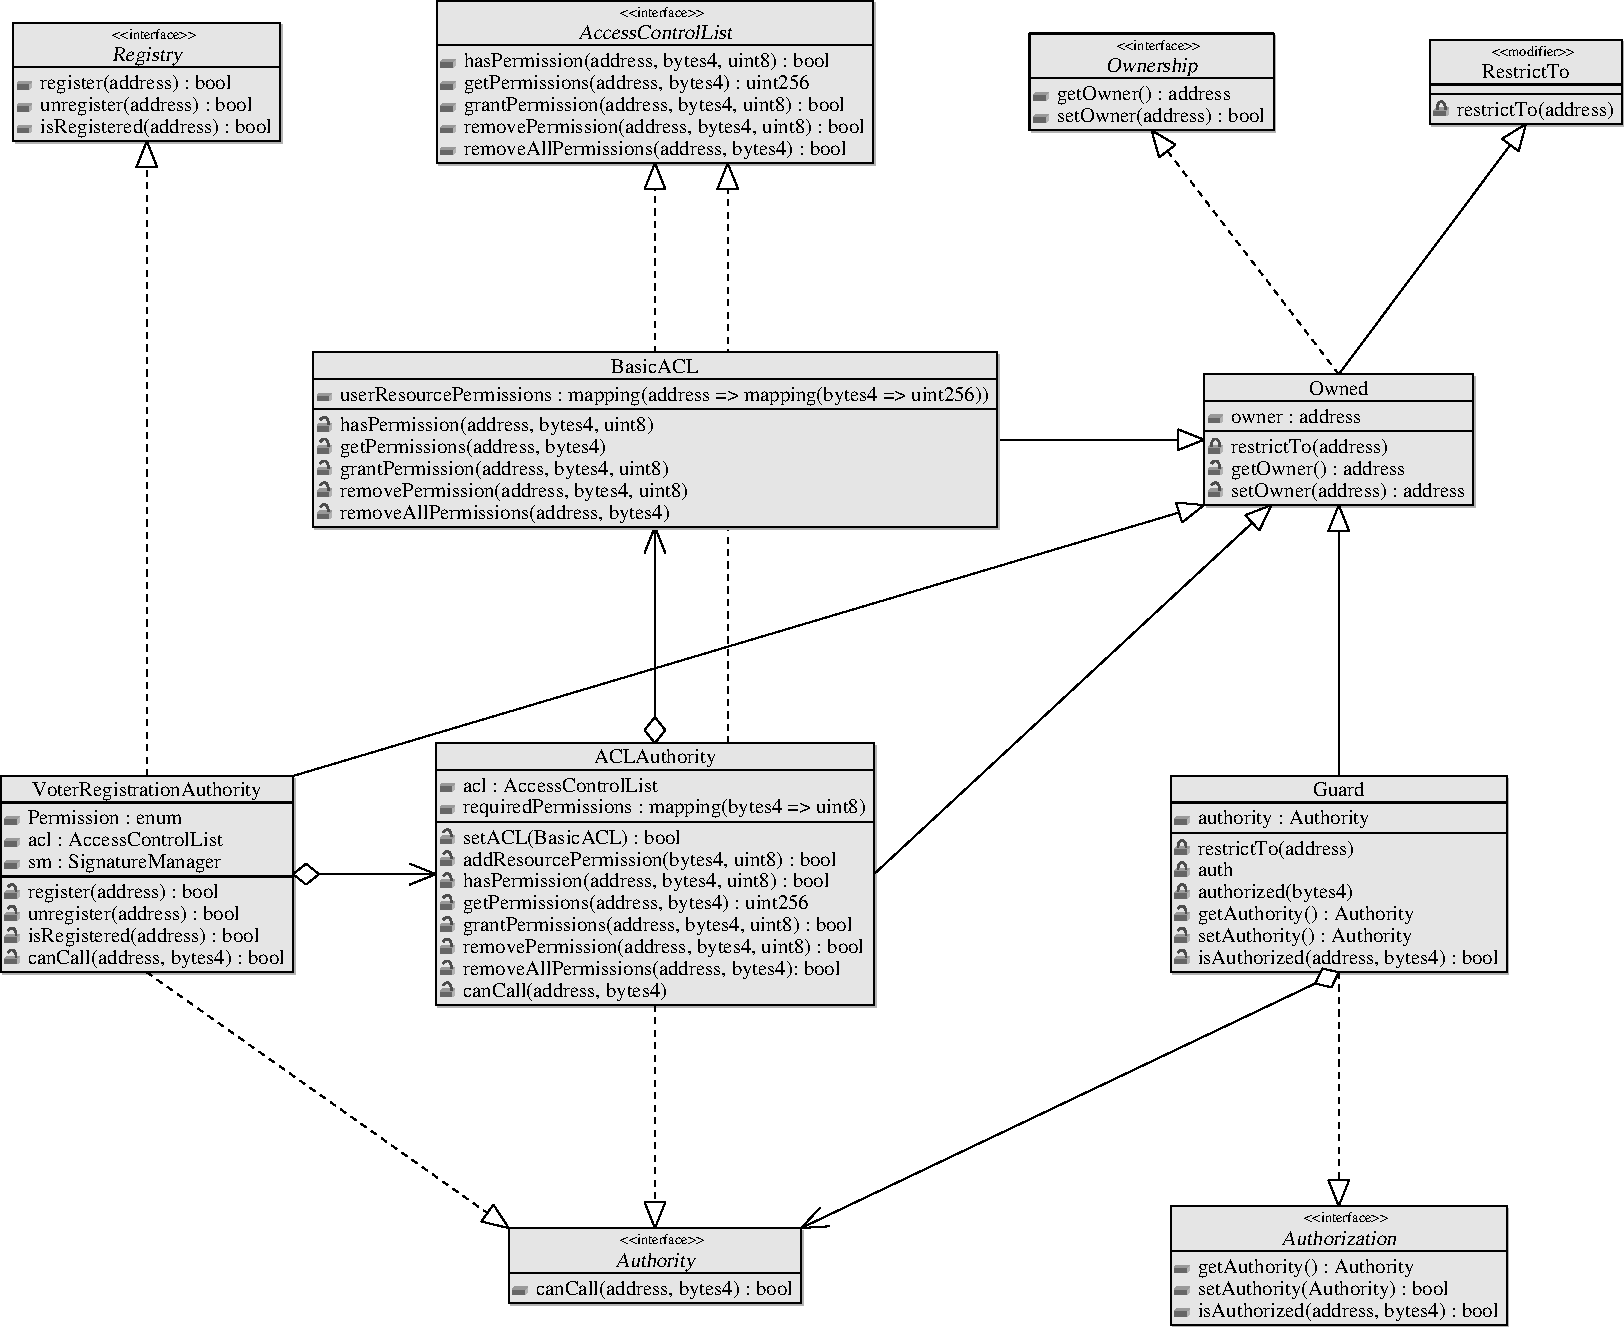
\includegraphics[width=\textwidth]{figures/authorization/figure}
    % \includestandalone[width=\textwidth]{\fig{authorization}}
    \caption{DVBM System Architecture~\cite{dc-voting-system}}\label{fig:dvbm-architecture}% \label{fig:authorization}
\end{figure}

Prior to the official launch of the system the BOEE opted to conduct a mock
election where members of the public, researchers, and hackers alike were
invited to to test the functionality of the system, discover vulnerabilities,
and attempt to compromise the security, reliability, and availability of the
system.\cite{internet-voting-survey,dc-voting-system,trust-the-vote-dc-pilot}

% \paragraph{Outcome}
Within 48 hours of the system going live researchers from The University of
Michigan, playing the role of an attacker, demonstrated a number of
vulnerabilities and attacks on on the system and managed to gained near-complete
control of the election server. Their intrusion was not detected for nearly 2
days.\cite{dc-voting-system}
% Prior to its launch election officials held a mock election to test the security
% of the system, inviting researchers and hackers alike to attempt to compromise
% the security, reliability, and availability of the system. A number of attacks
% were demonstrated and researchers were able to:

Demonstrated vulnerabilities included being able to:
\begin{itemize}
  \item penetrate the network of the election software
  \item determine voter's identities
  \item locate unencrypted ballots, thus mapping voter's identities to their
    personal votes
  \item modify ballots
  \item cast fake ballots
  \item modify the election system software itself
\end{itemize}

Once election officials became aware of the attack, the mock election was
suspended, five days ahead of schedule, citing ``usability issues.'' Election
officials later confirmed that they were unable to detect the attack or network
presence using their intrusion detection system. Due to the test results, the
portion of the system which allowed for ballots to be submitted over the
Internet was not used.\cite{dc-voting-system}

\subsubsection{Estonia --- 2005}
Estonia began using Internet voting in 2005\cite{internet-voting-survey}; in the
2015 Estonian parliamentary elections, 30.5\% of all voters voted over the
Internet. Estonia maintains what is likely the most advanced national
identification cards in the world. Estonian IDs are part of a \emph{Public Key
Infrastructure (PKI)} where IDs serve as smart cards which possess two RSA key
pairs: one for signing and one for authentication; these cryptographic functions
are performed directly on the card. The signatures produced by these IDs are
used extensively throughout the country and are considered legally binding.
These cryptographic IDs allow Estonia to provide voter authentication
capabilities that cannot be reproduced in the US.\ Despite the advanced
authentication capabilities that Estonia is able to achieve, researchers in 2014
devised a number of attacks that could be performed on the Estonian voting
system to spoil ballots, damage ballot secrecy, and steal or drop votes. The
researchers also criticized the transparency and operational security of the
system, noting that videos of the administration processes --- provided for
transparency purposes --- recorded administrators entering root passwords,
revealed network credentials which had been posted on a wall, and showed
administrators using USB drives containing personal files to move sensitive
election materials between systems.\cite{estonia}

% \subsection{Shared Weaknesses}\label{section:shared-weaknesses}
% There are a number of shared weaknesses and vulnerabilities exposed across these
% internet voting systems which the systems incur due to the underlying
% architecture of the systems, their Internet, the personal computer, and remote
% voting.
%
% \begin{enumerate}
%   \item Lack of voter-verified audit trails.
%   \item Vulnerabilities to insider attacks.
%   \item Privacy.
%   \item Vote Buying/Selling.
%   \item Intimidation.
%   \item Large-Scale Impact.
%   \item Too Many Potential Attacks.
%   \item Many Sources of Attacks.
%   \item Undetectable Attacks.
%   \item On-screen Electioneering.
% \end{enumerate}

% \todo{
%   Should I add a shared weaknesses section here and remove some of the
%   demonstrated attacks from the individual systems?
% }


% Section: End-to-End Verifiability
\section{End-to-End Verifiability}\label{sec:e2e-viv}
The vulnerabilities and weaknesses of electronic voting systems demonstrate a
clear need for a stronger kind of system design. \emph{End-to-End Verifiable
(E2E-V)} voting systems are systems which aim to provide such a design by
providing the following features for voters:

\begin{enumerate}
  \item allows voters to check that the system recorded their votes correctly

  \item allows voters to check that the system included their votes in the final
    tally

  \item allows voters to count the recorded votes and double-check the announced
    outcome of the election.
\end{enumerate}

% E2E-V voting systems have been a hotbed of research over the past several years.
An \emph{End-to-End Verifiable Internet Voting (E2E-VIV)} is an E2E-V voting
system that supports voting over the Internet.

% \begin{displayquote}
%    Aggressive early adoption of election technology must be tempered by a clear
%    understanding that voters’ trust in their elections is hard-won and easily
%    lost.
% \end{displayquote}


\subsection{Requirements}
In 2015, the U.S. Vote Foundation published a specification and feasibility
assessment study which laid out requirements for building an end-to-end
verifiable internet voting system. The study broke these requirements into two
categories:\cite{e2e-viv}

\begin{itemize}
  \item \emph{Technical Requirements}, the set of requirements which can be
    directly addressed by system design and architecture

  \item \emph{Non-Functional Requirements}, the set of requirements which must
    be imposed on a system by external entities
\end{itemize}

% cite: The Future of Voting: E2E-VIV
% This section reviews those requirements.

\subsubsection{Technical Requirements}
The ten categories of technical requirements, those which should be addressed
by the design and architecture of the systems itself, are:\cite{e2e-viv}

\begin{enumerate}
    \item functional requirements
    \item accessibility requirements
    \item usability requirements
    \item security requirements
    \item authentication requirements
    \item auditing requirements
    \item system operational requirements
    \item reliability requirements
    \item interoperability requirements
    \item certification requirements
\end{enumerate}

% \paragraph{Functional}
% \begin{displayquote}
%   The functional requirements of an E2E-VIV system deal primarily with the
%   casting and recording of ballots and associated voter records.
% \end{displayquote}

The \emph{functional requirements} deal primarily with casting and recording of
ballots. \emph{Receipt freedom} is one such functional requirement. An
electoral system which expresses receipt freedom is said to make it impossible
for a voter to prove to anyone how they voted.
%
% \subparagraph{Receipt freedom} is one such functional requirement, a property
% where it is impossible for a voter to prove to anybody how they voted.
%
Others functional requirements include:
\begin{itemize}
    \item ensuring that a voter cast a ballot if such an act is recorded
    \item data retention in case of failure
    \item multi-vote functionality to overwrite previous votes
    \item maintaining voter anonymity
\end{itemize}

% \paragraph{Usability}
% \begin{displayquote}
%   The usability of an E2E-VIV system is critical to its successful adoption and
%   use.
% \end{displayquote}

\emph{Usability} is mostly concerned with user experience and confirmation
guarantees. For example, voters should be confident that their vote was cast by
being provided a confirmation screen. The voting process should be both
intuitive and guide the voter through the process. Presentations such as the
butterfly ballot should be avoided at all costs.

% \paragraph{Accessibility}
% \blockquote{\emph{Accessibility} is the property of being usable by and
% useful to voters with disabilities.}

Digital voting systems have the potential to provide wider \emph{accessibility}
guarantees than traditional paper ballots for voters with disabilities. To
provide these guarantees developers must involve voters throughout the
development process to identify accessibility issues and implement solutions.

% \paragraph{Security}
\emph{Security} is an integral property and requirement which voting systems
must maintain. Included in this requirement is that:

\begin{itemize}
    \item no data can be permanently lost
    \item integrity of voters, candidates, ballot information, cast ballots, and
      other critical information must be maintained
    \item accurate timing information is critical for auditing
    \item voting equipment must be protected
    \item the system must perform regular health checks
\end{itemize}

% \paragraph{Authentication}
\emph{Authentication} is the process of ascertaining the validity of a claimed
identity. Authentication ensures that the voting system can enforce privacy and
prevent multi-voting, Sybil attacks, and vote theft. All individuals must be
identified uniquely. The system must allow access to services only to authorized
users, e.g., only allow election officials to load ballot info.

% \paragraph{Auditing}
The property of \emph{auditability} means that a voting system is capable of
comprehensive examination. Auditability must exist at all stages and levels of
the voting process. The system must keep auditable logs of all relevant activity
and the logs must be public and write only. Furthermore, the logs cannot leak
any data regarding voters or the way any ballot was cast. Privacy must always
be the foremost concern.

The auditing system must actively report issues and information in
real-time. At least the following events should be recorded:\cite{e2e-viv}
\begin{itemize}
  \item ``all voting-related information, including the number of eligible
    voters and votes cast, the number of invalid votes, count and recount
    results, etc.''
  \item ``any detected attacks on the operation of the system or its
    communication infrastructure''
  \item ``any system failures, malfunctions, or other detected threats to proper
    system operation.''
\end{itemize}
%
% \blockquote[{\cite[67]{}}]{%
%     \begin{itemize}
%         \item all voting-related information, including the number of eligible voters and
%             votes cast, the number of invalid votes, count and recount results, etc.;
%         \item any detected attacks on the operation of the system or its communication
%             infrastructure; and
%         \item any system failures, malfunctions, or other detected threats to proper
%             system operation.
%     \end{itemize}
% }
%
The system should provide auditing features which support the ability to:\cite{e2e-viv}
\begin{itemize}
  \item ``cross-check and verify the correct operation of the voting system and
    the accuracy of the election results''
  \item ``detect voter fraud''
  \item ``prove that all counted votes are legitimate and that all ballots have
    been counted''
\end{itemize}
%
% \blockquote[{\cite[67]{}}]{%
%     \begin{itemize}
%         \item cross-check and verify the correct operation of the voting system and the
%             accuracy of the election results;
%         \item detect voter fraud; and
%         \item prove that all counted votes are legitimate and that all ballots have been
%             counted.
%     \end{itemize}
% }
%
Finally, auditability must extend to the source code, actions performed, and the
documentation itself.

% \paragraph{System Operational}
\emph{System operational} requirements are those that enforce and regulate
transparency, accountability, system configuration, and updates. Logs, software,
configurations, versions, updates, etc., must all be managed and produced to
audit for tampering. Protocols should be in place to guard sensitive equipment
at all times and handle system failures. Officials managing these systems and
the procedures themselves must be scrutinized closely to prevent insider attacks
and election fraud.

% \paragraph{Reliability}
\emph{Reliability} is the property of a system behaving reasonably and as
expected under both normal conditions and while under attack. During an election
period a system should be highly available. 99.9\% availability is a minimum for
voting systems. The system must also be able to recover from any failure within
10 minutes, with the exception for failure caused by natural disaster or
malicious attack. The system should have redundant backup systems for critical
components of the system.

Internet voting systems are compelling targets for Distributed Denial of Service
(DDoS) attacks, therefore it is important that an E2E-VIV system be hardened to
such attacks and be able to continue operation with full correctness during a
sustained DDoS attack.

% \paragraph{Interoperability}
An E2E-VIV system must use open standards for \emph{interoperability} between
components, services, and other E2E-VIV systems. Logs and documentation of such
standards must be published so that anyone can download, inspect, and publish
analysis and concerns.

% \paragraph{Certification}
Finally, there should be \emph{certification} and test procedures involved for
every functional requirement; these tests should be able to be run on demand.
Formal proofs of security and correctness should be provided wherever possible,
and third-parties should be hired to conduct an independent review, audit, and
test of the system.

\subsubsection{Non-functional Requirements}
The five non-functional requirements defined, those which must be fulfilled by
external entities, e.g., operators and administrators, are:\cite{e2e-viv}

\begin{enumerate}
    \item operational requirements
    \item procedural requirements
    \item legal requirements
    \item assurance requirements
    \item maintenance/evolvability requirements
\end{enumerate}

% \paragraph{Operational}
The specification describes several \emph{operational} requirements: election
and registration timing, maintaining voter registration and candidate
nomination lists, providing receipt freedom, voter assistance, election
integrity, and openness.

% \subparagraph{Voter Assistance}
Voters must be well-informed on how to register, vote, and protect their privacy
in the voting system.
% \subparagraph{Election and Registration Timing}
Clear instruction on when voting and registration occurs should be announced far
in advance for the voter's benefit. When multiple forms of remote voting take
place, votes cast over the Internet should not be accepted after other forms of
remote voting end.
% \subparagraph{Voter Registration}
E2E-VIV systems must publish a voter register that is regularly updated. Voters
should be able to check that information in the register is accurate and request
corrections.
% \subparagraph{Candidate Nomination Lists}
The ballot presented to voters must be consistent, fair, unbiased, and free from
any superfluous information about candidates/choices.

% \subparagraph{Receipt Freedom}
Operational receipt freedom represents two different requirements depending on
whether a voter is voting from a supervised or unsupervised location. In a
supervised location receipt freedom requires that the voting terminal clear all
indication of how a ballot was cast and ensure that no paper trail representing
how the ballot was cast is able to leave the polling place (except by official
means). In an unsupervised location any visual proof of vote should not be able
to be used to determine how a vote was cast or will be tallied.

% \subparagraph{Election Integrity}
If test ballots are capable of being submitted then those ballots must be
clearly marked as a test ballot with instruction on how to cast a real ballot.
The voting system should not disclose any results to any person until after the
voting period has ended, including alternative forms of voting. Tallying should
be done as soon as possible afterwards and the tallying process should be
transparent, recorded, and be able to be replayed. Any irregularities which
affect the integrity of votes should be recorded.

% \subparagraph{Openness}
An E2E-VIV system must be open and function properly regardless of the hardware
or software being used to run the voting software. The system must be available
for auditing by external actors, especially when considering components which
are expected to be run on external systems or voter's machines.

% \paragraph{Procedural}
\emph{Procedural} requirements define the processes required to deploy and run
the E2E-VIV system.

\begin{itemize}
  \item Procedures should be published regarding provisioning, certification,
    maintenance, availability, and use. For example, when updates occur,
    election officials must call upon an independent body to perform
    verifications of performance and certification of intent.

  \item Procedures should be in place to teach voters the voting process.

  \item Election officials should have maintenance and security procedures to
    ensure that voting equipment is operating nominally and has not been
    tampered with. For example, conducting sensitive operations should require
    teams of at least two people.

  \item As much as possible there should be procedures in place to allow
    observers to watch election procedures.

  \item Procedures should be in place to update results in the event that a
    voter proves that their vote was not accurately received or counted.
\end{itemize}

% \paragraph{Legal}
The \emph{legal} requirements include national, state, and local laws that apply
to voting systems, e.g., accessibility, anonymity, and availability guarantees.
Any deployed E2E-VIV system must comply with these laws. For example, election
officials must ensure that only one ballot by each voter is tallied when
multiple means of voting exist, e.g., remote and traditional polling place.
%
% Voters must be able to restart, discard, or alter their votes at any point
% during the voting process. The system must allow the voter to participate in an
% election without marking choices, i.e., casting blank or partially blank
% ballots. The voting system must always preserve anonymity and indicate clearly
% that the voters ballot has been cast and voting procedure completed.
%
\begin{displayquote}
  ``There must be no impediments to interested parties who want to study the
  E2E-VIV system. In particular, no nondisclosure agreement or contract of any
  kind may be required for download and study of, or for building, testing and
  publishing test results for, the E2E-VIV system.''\cite{e2e-viv}
\end{displayquote}
% \blockquote{There must be no impediments to interested parties who want to study
% the E2E-VIV system. In particular, no nondisclosure agreement or contract of any
% kind may be required for download and study of, or for building, testing and
% publishing test results for, the E2E-VIV system.}

% \paragraph{Assurance}
To meet \emph{assurance} requirements, client-side software must be functional
and free of bugs across a wide range of hardware and software stack
combinations. There must be strong security with respect to authentication such
that voter credentials cannot be forged or invalidated without breaking
underlying cryptographic protocols.

The entirety of the voting system --- e.g., software, documentation, design,
architecture, algorithms, build scripts, issue tracking system, etc. --- must be
free, open, and public. All available resources should be up to date, certified,
and released under license that permits anyone to download, build, test, or
modify the source.

% \paragraph{Maintenance and Evolvability}
To meet \emph{maintenance and evolvability requirements} election officials must
have the right and ability to update the election system to conform to law,
technology, or threat independent of the original vendor.

\subsection{Architecture}
% \todo{Improve the Architecture content.}
The study, ``The Future of Voting: End-to-End Verifiable Internet Voting,''
provides an architectural feature model, seen in Figure~\ref{fig:viv-model},
which defines over 127,000 possible architectural variants.\cite{e2e-viv}

\begin{figure}[H]
  \setstretch{1}
  \begin{Verbatim}[
    label={[Architectural Feature Model]Architectural Feature Model},
    tabsize=2,
    fontsize=\scriptsize,
    frame=lines,
    framesep=5mm,
    numbers=left,
    fillcolor=\color{yellow}
  ]
  -- This diagram shows the various dimensions of an E2EVIV architecture
  static_diagram E2EVIV_Architecture_Dimensions
  component
    class E2EVIV_ARCHITECTURE
    feature
      authority_distribution: SET[VALUE]
        ensure 0 < Result.count;
          for_all v: VALUE such_that v member_of Result
            it_holds v member_of { Centralized, Distributed };
        end
      crypto_protocols: SET[VALUE]
        ensure 0 < Result.count;
          for_all v: VALUE such_that v member_of Result
            it_holds v member_of { On_Paper, Mechanized, Verified, Generated };
        end
      correctness_evidence: SET[VALUE]
        ensure 0 < Result.count;
          for_all v: VALUE such_that v member_of Result
          it_holds v member_of { Process_Based, Assertions };
        end
      implementation_type: SET[VALUE]
        ensure 0 < Result.count;
          for_all v: VALUE such_that v member_of Result
            it_holds v member_of { Golden_Implementation, Open_Protocols_and_Specs };
        end
      key_distribution_method: SET[VALUE]
        ensure 0 < Result.count;
          for_all v: VALUE such_that v member_of Result
            it_holds v member_of { Public_Ceremony, Threshold_Cryptography, PKI, Web_of_Trust };
        end
      deployment_style: SET[VALUE]
        ensure 0 < Result.count;
          for_all v: VALUE such_that v member_of Result
            it_holds v member_of { Trusted_Servers, Public_Cloud, Peer_to_Peer };
        end
      client_technology: SET[VALUE]
        ensure 0 < Result.count;
          for_all v: VALUE such_that v member_of Result
            it_holds v member_of { Custom_App, Web_Based };
        end
    end
  end
  \end{Verbatim}
  \caption{A specification of the possible variants for an E2E-VIV system.\cite{e2e-viv}}\label{fig:viv-model}
\end{figure}

Most of the variability available when constructing an E2E-VIV system stems from
the cryptographic techniques and tools available to select from when designing
the system.

\subsubsection{Cryptographic Techniques and Tools}
The cryptographic techniques and cryptosystems available for use in E2E-V
electoral systems are presented in this section; this is not a comprehensive
list of cryptographic techniques and tools available, but includes some of the
most common techniques and tools leveraged in E2E-VIV systems.

% \paragraph{Asymmetric Cryptography}
Asymmetric cryptography, also known as public-key cryptography, uses pairs of
keys to securely encrypt and decrypt messages. There are many different
public-key based cryptosystems available for use.

% \paragraph{Homomorphic Schemes}
Homomorphic cryptographic schemes allow one to perform basic arithmetic
operations on ciphertexts without requiring decryption of the ciphertext. This
property has a number of uses in E2E-VIV systems; for example, an E2E-VIV system
might leverage this property to tally a collection of encrypted ballots without
decrypting any individual's ballots.

% \subparagraph{Additive Homomorphic Encryption}
Additive homomorphic encryption schemes enable processing of ciphertexts by way
of addition. The Pallier and Benaloh cryptosystems both support additive
homomorphic encryption.\cite{helios}

% \subparagraph{Multiplicative Homomorphic Encryption}
Multiplicative homomorphic encryption schemes enable processing ciphertexts by
way of multiplication. The ElGamal cryptosystem supports multiplicative
homomorphic encryption.

% \paragraph{Append-Only Public Bulletin Board}
Most E2E-VIV systems depend on an append-only web/public bulletin
board.\cite{bulletin-board} The append-only public bulletin board is a
publicly-visible secure location where election operations and ballot data are
submitted, logged, and made available to support auditing
requirements.\cite{e2e-viv,helios,almost-correct-mixing,pretty-good-democracy,mix-networks,vector-ballot-voting}
Blockchains fulfill most of the requirements of an append-only public bulletin
board.

% \subsubsection{Secret Sharing and Threshold Schemes}
Secret sharing and threshold schemes allow a collection of actors to cooperate
to produce ``shares'' of a secret; each participant is responsible for
managing their share of the secret and some threshold of shares must come
together to recover the complete secret or perform cryptographic
operations.\cite{distributed-key-generation,large-scale-distributed-key-generation}

% \paragraph{Zero-Knowledge Proofs}
A zero-knowledge proof (ZKP) is a probabilistic method which allows one party
to prove knowledge of some secret without revealing any information about the
secret itself. A zero-knowledge proof satisfies the following properties:\cite{e2e-viv,zkproof}
%
\begin{enumerate}
  \item Completeness, an honest verifier will be convinced by an honest prover.
  \item Soundness, an honest verifier will not be convinced by a dishonest
    prover.
  \item Zero-knowledge, the verifier will not learn any information regarding
    the secret itself.
\end{enumerate}
%
% \subparagraph{Non-Interactive Zero-Knowledge Proofs}
A useful form of zero-knowledge proofs are non-interactive zero-knowledge
proofs --- also known as NIZKs, zk-SNARKs, or zkSTARKs --- which are
zero-knowledge proofs which require no interaction between the prover and
verifier for the verifier to be convinced of
correctness.\cite{helios,almost-correct-mixing,vector-ballot-voting,mix-networks}

% \paragraph{Mixnet Schemes}
Mixnet schemes are used to provide anonymity. Mix networks are operated by a
set of trusted nodes, mix-servers, which consume messages --- typically
encrypted ballot data in the case of E2E-VIV systems --- from a set of
network-participants to produce a random permutation of the input messages.
Each node performs a ``mix'' operation on the incoming messages in such a way
that the output cannot be unscrambled and tied back to a network-participant
except by the node itself which is performing the mixing operation. Therefore,
as long as any single mix-server in the mix network is acting honestly, the
anonymity of the participants will be
maintained.\cite{mix-networks,vector-ballot-voting}

% \subparagraph{Decryption Mixnet}
A decryption mixnet operates by encrypting a message in multiple layers with
each mix server's public key. To decrypt the message, the message layers are
decrypted in the opposite order they were encrypted in by each node. Each node
forwards its decrypted results to the next node in the mix network. So long as a
single node does not reveal the source of the message then the message will
become untraceable (assuming no information is leaked by the message
itself).\cite{mix-networks}

% \subparagraph{Re-encryption Mixnet}
A re-encryption mixnet works by leveraging the re-encryption properties of the
underlying encryption scheme. Certain cryptosystems make it possible to change a
ciphertext without modifying the underlying message. In this way a set of nodes
can shuffle and re-encrypt a ciphertext then pass them to the next mixnet node
to repeat the process. So long as a single node does not reveal the shuffling
process the anonymity offered by the mixnet will be
maintained.\cite{mix-networks,almost-correct-mixing}

% \paragraph{Blind Signature Schemes}
Blind signature schemes separate the voter authentication, authorization, and
signing components from the vote tallying, shuffling, and decryption components.
A voter will encrypt a ballot (blind it) then send it to a signing authority who
will blind-sign the encrypted ballot after it has verified that the voter is
qualified to vote. Once a voter has acquired a blind signed ballot they can
strip their identifying data, unblind the ballot, and submit the signed ballot
through an anonymous channel. The underlying cryptosystem makes it such that the
blind signed ballot is equivalent to a signed unblinded ballot.\cite{e2e-viv}

% cite

% \paragraph{ElGamal}
% The ElGamal cryptosystem is a
%
% \paragraph{Paillier}

% \subsection{Existing Systems}
% \todo{Complete section.}
% \todo{Do not directly discuss any systems which are strictly physical.}

% \subsubsection{Estonia}
% Estonia began using Internet voting in 2005. By the 2015 Estonian parliamentary
% elections 30.5\% of all voters voted over the Internet. Estonia maintains what
% are probably the most advanced national identification cards in the world.
% Estonian IDs are part of a \emph{Public Key Infrastructure (PKI)} where IDs
% serve as smart cards which possess two RSA key pairs: one for signing and one
% for authentication. Cryptographic functions are performed on the card. The
% signatures produced by the IDs are used extensively throughout the country and
% are legally binding. These cryptographic IDs allow Estonia to provide voter
% authentication capabilities that cannot be reproduced in the US.\ Despite the
% advanced authentication capabilities that Estonia offers researchers in 2014
% devised a number of attacks that could be performed on the Estonian voting
% system to spoil ballots, damage ballot secrecy, and steal/drop votes. The
% researchers also criticized the transparency and operational security of the
% system.

% \subsubsection{Helios}
% \todo{Review Ben Adidas' Helios system.}

% \subsubsection{RIES}
% \todo{Complete section.}

% \subsubsection{Pret A Voter}
% \todo{Special characters/spelling in pret a voter.}

% \subsubsection{Punchscan}
% \todo{Complete section.}
%
% \subsubsection{Scantegrity II}
% \todo{Complete section.}

% \subsubsection{Remotegrity}
% \todo{Complete section.}

% \subsubsection{Norwegian System}
% \todo{Complete section.}

% \subsubsection{Wombat}
% \todo{Review Wombat.}
% \todo{Complete section.}

% \subsubsection{Demos}
% \todo{Complete section.}
% \todo{Review Demos.}

% \subsubsection{vVote}
% \todo{Complete section.}


% Section: Notable Voting Systems and Experiments
% % \section{Novel Electoral Systems, Voting Experiments, and Technologies}
\section{Notable Voting Systems \& Experiments}
What follows is a review of other notable voting systems and experiments:

\subsection{Novel Voting Systems}

\subsubsection{Estonia}
Estonia began using Internet voting in 2005. By the 2015 Estonian parliamentary
elections 30.5\% of all voters voted over the Internet. Estonia maintains what
are probably the most advanced national identification cards in the world.
Estonian IDs are part of a \emph{Public Key Infrastructure (PKI)} where IDs
serve as smart cards which possess two RSA key pairs: one for signing and one
for authentication. Cryptographic functions are performed on the card. The
signatures produced by the IDs are used extensively throughout the country and
are legally binding. These cryptographic IDs allow Estonia to provide voter
authentication capabilities that cannot be reproduced in the US.\ Despite the
advanced authentication capabilities that Estonia offers researchers in 2014
devised a number of attacks that could be performed on the Estonian voting
system to spoil ballots, damage ballot secrecy, and steal/drop votes. The
researchers also criticized the transparency and operational security of the
system.

\subsection{Blockchain Voting Systems}
\todo{Compare and contrast other electoral systems with this research, discuss
weaknesses, holes in the research, etc.}

% \subsection{Voting Machines}
% \todo{Complete section.}
%
% % #### Diebold AccuVote-TS
% \subsubsection{Diebold AccuVote-TS}
% \todo{Complete section.}
%
% % #### AVS WINVote
% \subsubsection{AVS WINVote}
% \todo{Complete section.}

% \subsection{Voting Experiments}

% ### Demonstrated Attacks
% The following is a review of Internet voting systems that research has shown to
% be susceptible to attack.


% \subsection{Voting Technologies}

% ### Demonstrated Attacks
% The following is a review of electronic voting machines that research has
% shown to be susceptible to attack.
%
% \subsection{Compare and Contrast}

% \todo{Add back the Novel Electoral Systems section once it has been improved.}

% Section: Ethereum
% \subsection{Ethereum}

Ethereum is a blockchain-based system initially proposed in late 2013,
post-Bitcoin, and released in 2015.\cite{ethereum-white} Ethereum introduced a
few novel features and functionalities with its blockchain network which are not
available in the Bitcoin network. Most notably Ethereum offers a distributed
decentralized Turing-complete computing platform via the Ethereum Virtual
Machine (EVM), which aims to provide an application layer which ``[runs] exactly
as programmed without any possibility of downtime, censorship, fraud or third
party interference.''\cite{ethereum.org,ethereum-yellow}

\subsubsection{Fundamental Concepts}

\paragraph{Currency}
Like Bitcoin, Ethereum's blockchain defines and leverages its own token,
\solt{ether} --- also referred to as \solt{eth} or ETH, and sometimes denoted
using the Greek symbol Xi, $\Xi$, the uppercase Old English letter Eth, \DH, or,
more rarely, $\blacklozenge$ --- which acts as the underlying currency of its
blockchain protocol. The smallest unit of \solt{ether} is
\emph{wei}.~\cite{mastering-ethereum,ethereum-yellow} The
denominations of \solt{ether} are broken down as follows:
% \ref{book:mastering-ethereum}
% \ref{paper:ethereum}

% \todo{Add denomination table here}

% \ref{book:mastering-ethereum}
% \ref{paper:ethereum}
%
% See page 2 of Ethereum yellow paper.
%
% Table 2-1 from page 14 of Mastering Ethereum.
%
% | Value (in wei) | Exponent | Common Name | SI Name               |
% |----------------|----------|-------------|-----------------------|
% | 1              | 1        | wei         | Wei                   |
% | 1000           | 10^3     | Babbage     | Kilowei or femroether |
% |                |          |             |                       |
% |                |          |             |                       |

\begin{center}
    \setstretch{1.5}
    \footnotesize
    \begin{longtabu} to \textwidth{@{} X[3] X[] X[] X[2] @{}}
    \caption{Ether Denominations~\cite{mastering-ethereum}}\label{tab:eth-denominations} \\
    \toprule
    Value (in wei)                    & Exponent & Common Name & SI Name \\
    \midrule
    \endfirsthead
    \toprule
    Value (in wei)                    & Exponent & Common Name & SI Name \\
    \midrule
    \endhead
    \taburowcolors{white..gray!15}
    1                                 & $10^{0}$    & wei       & Wei \\
    1,000                             & $10^{3}$    & Babbage   & Kilowei or femtoether \\
    1,000,000                         & $10^{6}$    & Lovelace  & Megawei or picoether \\
    1,000,000,000                     & $10^{9}$    & Shannon   & Gigawei or nanoether \\
    1,000,000,000,000                 & $10^{12}$   & Szabo     & Microether or micro \\
    1,000,000,000,000,000             & $10^{15}$   & Finney    & Milliether or milli \\
    1,000,000,000,000,000,000         & $10^{18}$   & Ether     & Ether \\
    1,000,000,000,000,000,000,000     & $10^{21}$   & Grand     & Kiloether \\
    1,000,000,000,000,000,000,000,000 & $10^{24}$   &           & Megaether \\

    %extern u256 const c_copyGas;			///< Multiplied by the number of 32-byte words that are copied (round up) for any *COPY operation and added.
    \bottomrule
    % \begin{varwidth}{\textwidth}
    %   These names pay homage to some of the great minds of cryptography and
    %   computer science.
    % \end{varwidth}
  \end{longtabu}
\end{center}

\paragraph{Accounts}
Accounts are an Ethereum primitive which provide an abstraction over the Bitcoin
equivalent signature chain process; this abstraction helps to both simplify the
concept of token ownership as well as extend the idea of what a token is, what a
token can be, and how blockchain state can be managed and organized.

Accounts are identified by a 160-bit code, their \solt{address}, and are
internally represented by four properties:

\begin{enumerate}
  \item \sol{nonce}, a monotonically increasing counter which represents the
    number of transactions sent from the account.
  \item \sol{balance}, the amount of \solt{ether}, expressed in wei, which is
    owned by the account.
  \item \sol{storageRoot}, a 256-bit hash of the root node of a Merkle Patricia
    tree which encodes the storage contents of the account.

    % RLP - Recursive Length Prefix
    % https://eth.wiki/en/fundamentals/rlp

    % https://blog.ethereum.org/2015/11/15/merkling-in-ethereum/
    %
    % From the yellow paper:
    % \displayquote{
    %   A 256-bit hash of the root node of a Merkle Patricia tree that encodes
    %   the storage contents of the account (a mapping between 256-bit integer
    %   values), encoded into the trie as a mapping from the Keccak 256-bit hash
    %   of the 256-bit integer keys to the RLP-encoded 256-bit integer values.
    %   This tree encodes the hash of the storage contents of this account, and
    %   is empty by default.
    % }


  \item \sol{codeHash}, an immutable hash of the EVM code corresponding to the
    account.
\end{enumerate}

Although all accounts are structurally identical it is useful to distinguish
between the two practical kinds of accounts which one is likely to encounter and
interact with on the Ethereum blockchain, \emph{external accounts} and
\emph{internal accounts}:
%
\begin{description}[font=\normalfont\emph]
  % \subsubparagraph{External Accounts}
  \item[External Accounts] --- also referred to as simple accounts, non-contract
    accounts, externally owned accounts (EOA), and sometimes user accounts ---
    are defined as accounts whose \sol{codeHash} value is the Keccak-256 hash of
    an empty string; i.e., the account contains no code.

  %\subsubparagraph{Internal Accounts}
  \item[Internal Accounts] --- also referred to as contract accounts --- are
    those accounts which are not external accounts; i.e., the account contains
    code.
\end{description}
%
Both kinds of accounts have the ability to send and receive \solt{ether} as well
as interact with \solt{contract}[s] which have been deployed to the Ethereum
network. However, there are some key differences between the two kinds of
accounts which are worth highlighting:\cite{ethereum:accounts}

\begin{itemize}[label=]
  \item External Accounts
    \begin{itemize}[label=$\bullet$]
      \item External accounts are managed by public-key cryptography.
      \item External account creation costs no \solt{ether}.
      \item Only external accounts can \emph{initiate} transactions.
      \item Transactions between external accounts can only transact
        \solt{ether}.
    \end{itemize}
  \item Internal Accounts
    \begin{itemize}[label=$\bullet$]
      \item Internal accounts are managed by code.
      \item Internal account creation costs \solt{ether} which reflects the cost
        of storing code on the Ethereum network.
      \item Internal accounts can execute code via the EVM upon receiving
        transactions, enabling a wide range network functionalities.
      \item Internal accounts can only send transactions in response to
        receiving transactions. \todo{This will have a major impact on the
        methodologies.}
    \end{itemize}
\end{itemize}

\paragraph{Transactions}
A transaction is a cryptographically-signed instruction constructed by an
external actor and submitted to the Ethereum network. There are two kinds of
transactions worth distinguishing, contract creation transactions and message
call transactions; both kinds of transactions share the following common
properties:

\begin{enumerate}
  \item \sol{to}, a 160-bit \solt{address} representing the \emph{recipient's}
    account. This value is omitted when building a contract creation
    transaction.

  \item \sol{from}, a signature which identifies the \emph{sender} of the
    transaction by account \solt{address}.\footnotemark{}

    \footnotetext{
      This field does not \emph{technically} exist, in actuality the signature
      is represented as three distinct fields (\emph{v}, \emph{r}, \emph{s}),
      which can be used to determine the \solt{address} representing the sender
      of the transaction.
    }

  \item \sol{value}, the amount of \solt{ether}, expressed in wei, which is
    to be transferred to the recipient.

  \item \sol{nonce}, a value equal to the number of transactions which have been
    sent by the \emph{sender}.

  \item \sol{gasPrice}, a value representing the amount of wei to be paid per
    unit of gas (expanded on below).

  \item \sol{gasLimit}, a value representing the maximum amount of gas which
    should be used executing the transaction.
\end{enumerate}

Contract creation transactions include the following additional property in the
transaction:

\begin{enumerate}
  \item \sol{init}, an EVM-code fragment which is executed only once and
    discarded thereafter; it returns the \sol{body}, a second fragment of code
    that executes each time the account receives a message call, which can occur
    either by transaction or internal execution of code.
\end{enumerate}

In contrast, a message call transaction includes the following additional
property:

\begin{enumerate}
  \item \sol{data}, an unlimited size byte array which contains the input data
    of the message call.
\end{enumerate}

\paragraph{Ethereum Virtual Machine}\label{eth:evm}
The Ethereum Virtual Machine (EVM) is the execution environment which Ethereum
code is processed in. The EVM processes low-level bytecode and takes actions
against the state of the Ethereum blockchain in response: reading, processing,
and writing data. The Ethereum Virtual Machine Specification introduces a
low-level instruction set which defines the available operations which an EVM
implementation should support: the opcodes, their inputs, outputs, and various
other implementation details. The EVM can be described as a \emph{state
transition function}, $Y(S, T) = S'$; given a set of transactions, $T$, and an
initial state, $S$, the state transition function, $Y(S, T)$, will produce a new
output state, $S'$.\cite{ethereum-yellow} Several EVM implementations exist
which have been written in various languages, e.g., Go, Python, and C++.

\subparagraph{Language Support}\label{eth:languages}
Several higher-level languages exist which target the Ethereum Virtual Machine
and can be used to build ``smart contracts;'' e.g., Solidity which draws
inspiration from C++ and JavaScript, and Vyper which describes itself as a
``Pythonic Smart Contract Language.'' These languages ship with compilers which
can be used to translate their code into low-level EVM bytecode; Solidity, for
example, is compiled using \solt{solc}, the Solidity compiler.

% \subsubsection{Network Topology}
\subsubsection{Network Topology}
Like Bitcoin, Ethereum exists as a network of nodes, each node supporting
differing functionalities, which work collectively to construct the Ethereum
blockchain and support the surrounding ecosystem. These nodes can be classified
by the functionalities which they support.

\paragraph{Node Types}
There exists several implementations of the Ethereum protocol, i.e., Ethereum
clients, which have been written in various languages, e.g., Geth in Go, Parity
in Rust, and pyethereum in Python. Some of these clients support running in
different modes.

\begin{itemize}
  \item A \emph{full node} is a complete implementation of the Ethereum
    protocol. A full nodes processes and validates all transactions which have
    been added to the Ethereum blockchain, thus helping to support the
    resiliency and reliability of the network. To support this functionality, a
    full node must maintain a complete copy of the blockchain. Full nodes are
    also capable of deploying and interacting with contracts, support mining and
    wallet functionality, and are able to route transactions throughout the
    network.

  \item A \emph{remote client} supports a subset of the functionality that a
    full node supports, generally wallet functionality and the ability to
    broadcast transactions. Other more complex functionalities generally require
    interacting with with a full node or other remote services which are capable
    of fulfilling requests on a remote client's behalf.
\end{itemize}

\paragraph{The Blockchain}
Like Bitcoin, the Ethereum blockchain is constructed by leveraging a
Proof-of-Work (PoW) algorithm to reach consensus throughout the network. The
proof-of-work algorithm leveraged by Ethereum, Ethash, helps to build trust and
reliability throughout the network while also securing the blockchain and
ensuring that EVM code execution has been processed and that the results
produced from said execution are as expected. Ethereum offers cryptoeconomic
incentivization in the form of \solt{ether} to promote participation in the
proof-of-work process.\cite{ethereum-yellow}

\subparagraph{Blocks}
The Ethereum protocol groups collections of transactions into \emph{blocks}.
Blocks are linked to previous blocks, via cryptographic hash, which reflect the
prior states of the blockchain. When processed collectively these blocks reflect
the current state of the Ethereum blockchain.

\subparagraph{Proof-of-Work}
Ethereum's proof-of-work algorithm, Ethash, is a proof-of-work algorithm which
was initially inspired by the Hashimoto and Dagger algorithms. The primary
motivation behind the Ethash algorithm was to produce a PoW algorithm which
would be resistant to application-specific integrated circuits (ASICs). The
primary mechanism leveraged to achieve ASIC-resistance lies in the algorithm's
memory-bound nature: a significant amount of memory, in addition to computation,
is required to correctly compute a proof-of-work solution. By requiring large
amounts of memory-bound operations the algorithm makes itself resistant to most
kinds of specialized memories and caches. Additionally, the memory requirements
are designed to grow and shift over time such that building rapid static caches
would become prohibitively expensive. In some sense the Ethash algorithm might
be better described as Proof-of-Memory.\cite{dagger-hashimoto,hashimoto,dagger}

The Ethereum network has been attempting to migrate away from Ethash to a
lower-cost consensus algorithm operating through Proof-of-Stake (PoS) but has
yet to complete the transition.

% Talk about the Greedy Heaviest Observed Subtree (GHOST) protocol.

\subparagraph{Gas}
In order to validate that EVM code has been executed, and executed as expected,
each full node on the network must recompute all transactions and whatever EVM
code those transactions have triggered when validating blocks. It is not
difficult to imagine how this might cause serious problems and introduce room
for exploitation within the network, \sol{while true { expensiveOperation() }}.
In order to address this the Ethereum specification introduces an abstraction,
\emph{gas}, which has a market-based value and must be paid by the
transaction-sender up-front when generating a transaction. Each operation
computed by the EVM has an associated gas-price and that gas price is ``paid''
to the node who successfully mints a block. If an insufficient amount of gas is
provided by the transaction-sender then the EVM will throw an out-of-gas (OOG)
exception: execution halts, the blockchain state is restored, and all gas
submitted is forfeited to the node. If an excess of gas is provided then any gas
remaining after transaction execution is refunded to the sender. When generating
a transaction on the Ethereum network the creator of the transaction has the
choice of defining how much wei they are willing to pay per unit of gas. Nodes
are incentivized to process transactions which offer more wei per unit of gas
relative to the rest of the transactions available for processing on the
network. Table~\ref{tab:gas-costs} introduces gas costs as defined by the
Ethereum Yellow Paper.


% Stuff about gas. What follows is a table of some gas costs as defined in the Ethereum
% yellow paper.

\begin{center}
  \setstretch{1.5}
  \scriptsize
  \begin{longtabu} to \textwidth{@{} X[1.1,l] X[0.5,r] X[7,l] @{}}
  \caption{Fee Schedule\cite{ethereum-yellow}}\label{tab:gas-costs} \\
  \toprule
  Name & Value & Description* \\
  \midrule
  \endfirsthead
  \toprule
  Name & Value & Description* \\
  \midrule
  \endhead
  \taburowcolors{white..gray!15}
  $G_{zero}$ & 0 & Nothing paid for operations of the set {\tiny $W_{zero}$}. \\
  $G_{base}$ & 2 & Amount of gas to pay for operations of the set {\tiny $W_{base}$}. \\
  $G_{verylow}$ & 3 & Amount of gas to pay for operations of the set {\tiny $W_{verylow}$}. \\
  $G_{low}$ & 5 & Amount of gas to pay for operations of the set {\tiny $W_{low}$}. \\
  $G_{mid}$ & 8 & Amount of gas to pay for operations of the set {\tiny $W_{mid}$}. \\
  $G_{high}$ & 10 & Amount of gas to pay for operations of the set {\tiny $W_{high}$}. \\
  $G_{extcode}$ & 700 & Amount of gas to pay for operations of the set {\tiny $W_{extcode}$}. \\
  $G_{balance}$ & 400 & Amount of gas to pay for a {\tiny BALANCE} operation. \\
  $G_{sload}$ & 200 & Paid for a {\tiny SLOAD} operation. \\
  $G_{jumpdest}$ & 1 & Paid for a {\tiny JUMPDEST} operation. \\
  $G_{sset}$ & 20000 & Paid for an {\tiny SSTORE} operation when the storage value is set to non-zero from zero. \\
  $G_{sreset}$ & 5000 & Paid for an {\tiny SSTORE} operation when the storage value's zeroness remains unchanged or is set to zero. \\
  $R_{sclear}$ & 15000 & Refund given (added into refund counter) when the storage value is set to zero from non-zero. \\
  $R_{selfdestruct}$ & 24000 & Refund given (added into refund counter) for self-destructing an account. \\
  $G_{selfdestruct}$ & 5000 & Amount of gas to pay for a {\tiny SELFDESTRUCT} operation. \\
  $G_{create}$ & 32000 & Paid for a {\tiny CREATE} operation. \\
  $G_{codedeposit}$ & 200 & Paid per byte for a {\tiny CREATE} operation to succeed in placing code into state. \\
  $G_{call}$ & 700 & Paid for a {\tiny CALL} operation. \\
  $G_{callvalue}$ & 9000 & Paid for a non-zero value transfer as part of the {\tiny CALL} operation. \\
  $G_{callstipend}$ & 2300 & A stipend for the called contract subtracted from $G_{callvalue}$ for a non-zero value transfer. \\
  $G_{newaccount}$ & 25000 & Paid for a {\tiny CALL} or {\tiny SELFDESTRUCT} operation which creates an account. \\
  $G_{exp}$ & 10 & Partial payment for an {\tiny EXP} operation. \\
  $G_{expbyte}$ & 50 & Partial payment when multiplied by $\lceil\log_{256}(exponent)\rceil$ for the {\tiny EXP} operation. \\
  $G_{memory}$ & 3 & Paid for every additional word when expanding memory. \\
  $G_\text{txcreate}$ & 32000 & Paid by all contract-creating transactions after the {\it Homestead transition}.\\
  $G_{txdatazero}$ & 4 & Paid for every zero byte of data or code for a transaction. \\
  $G_{txdatanonzero}$ & 68 & Paid for every non-zero byte of data or code for a transaction. \\
  $G_{transaction}$ & 21000 & Paid for every transaction. \\
  $G_{log}$ & 375 & Partial payment for a {\tiny LOG} operation. \\
  $G_{logdata}$ & 8 & Paid for each byte in a {\tiny LOG} operation's data. \\
  $G_{logtopic}$ & 375 & Paid for each topic of a {\tiny LOG} operation. \\
  $G_{sha3}$ & 30 & Paid for each {\tiny SHA3} operation. \\
  $G_{sha3word}$ & 6 & Paid for each word (rounded up) for input data to a {\tiny SHA3} operation. \\
  $G_{copy}$ & 3 & Partial payment for {\tiny *COPY} operations, multiplied by words copied, rounded up. \\
  $G_{blockhash}$ & 20 & Payment for {\tiny BLOCKHASH} operation. \\

  %extern u256 const c_copyGas;			///< Multiplied by the number of 32-byte words that are copied (round up) for any *COPY operation and added.
  \bottomrule
  \end{longtabu}
  % \begin{itemize} % [label=,leftmargin=0mm,topsep=0mm]
  \begin{multicols}{2}
    \begin{itemize}[label=,leftmargin=0mm,topsep=0mm,itemsep=0em]
      \scriptsize
      \item $W_{zero}$ = \tiny\{{STOP}, {RETURN}\}
      \scriptsize
      \item $W_{low}$ = \tiny\{{MUL}, {DIV}, {SDIV}, {MOD}, {SMOD}, {SIGNEXTEND}\}
      \scriptsize
      \item $W_{mid}$ = \tiny\{{ADDMOD}, {MULMOD}, {JUMP}\}
      \scriptsize
      \item $W_{high}$ = \tiny\{{JUMPI}\}
      \scriptsize
      \item $W_{extcode}$ = \tiny\{{EXTCODESIZE}\}
      \scriptsize
      \item $W_{base}$ = \tiny\{{ADDRESS}, {ORIGIN}, {CALLER}, {CALLVALUE},
        {CALLDATASIZE}, {CODESIZE}, {GASPRICE}, {COINBASE} {TIMESTAMP},
        {NUMBER}, {DIFFICULTY}, {GASLIMIT}, {POP}, {PC}, {MSIZE}, {GAS}\}
      \scriptsize
      \item $W_{verylow}$ = \tiny\{{ADD}, {SUB}, {NOT}, {LT}, {GT}, {SLT},
        {SGT}, {EQ}, {ISZERO}, {AND}, {OR}, {XOR}, {BYTE}, {CALLDATALOAD},
        {MLOAD}, {MSTORE}, {MSTORE8}, {PUSH*}, {DUP*}, {SWAP*}\}
    \end{itemize}
  \end{multicols}
\end{center}

% \paragraph{Transaction Examples}
% \subparagraph{Example 1: Alice to Bob}
% \subparagraph{Example 2: Alice to Contract}
% \subparagraph{Example 3: Contract to Contract}

